%%%%%%%%%%%%%%%%%%%%%%%%%%%%%%%%%%%%%%%%%%%%%%%%%%%%%%%%%%%%%%%%%%%%%%%%%%%%%%%%
% TUM-Vorlage: Wissenschaftliche Arbeit
%%%%%%%%%%%%%%%%%%%%%%%%%%%%%%%%%%%%%%%%%%%%%%%%%%%%%%%%%%%%%%%%%%%%%%%%%%%%%%%%
%
% Rechteinhaber:
%     Technische Universität München
%     https://www.tum.de
% 
% Gestaltung:
%     ediundsepp Gestaltungsgesellschaft, München
%     http://www.ediundsepp.de
% 
% Technische Umsetzung:
%     eWorks GmbH, Frankfurt am Main
%     http://www.eworks.de
%
%%%%%%%%%%%%%%%%%%%%%%%%%%%%%%%%%%%%%%%%%%%%%%%%%%%%%%%%%%%%%%%%%%%%%%%%%%%%%%%%


%%%%%%%%%%%%%%%%%%%%%%%%%%%%%%%%%%%%%%%%%%%%%%%%%%%%%%%%%%%%%%%%%%%%%%%%%%%%%%%%
\documentclass[%
    fontsize=11pt, % Schriftgröße
    twoside=off % kein einseitiges Layout
]{scrbook} % Dokumentenklasse: KOMA-Script Book
\usepackage{scrlayer-scrpage} % Anpassbare Kopf- und Fußzeilen

\usepackage[utf8]{inputenc} % Textkodierung: UTF-8
\usepackage[T1]{fontenc} % Zeichensatzkodierung

\usepackage[ngerman]{babel} % Deutsche Lokalisierung
\usepackage{graphicx} % Grafiken

% Schriftart Helvetica:
\usepackage[scaled]{helvet}
\renewcommand{\familydefault}{\sfdefault}

% Silbentrennung:
\usepackage{hyphenat}
\hyphenation{TUM in-te-res-siert} % Eigene Silbentrennung
%\tolerance 2414
%\hbadness 2414
%\emergencystretch 1.5em
%\hfuzz 0.3pt
%\widowpenalty=10000     % Hurenkinder
%\clubpenalty=10000      % Schusterjungen
%\vfuzz \hfuzz

\usepackage[hidelinks]{hyperref} % Hyperlinks
\usepackage[onehalfspacing]{setspace} % 1,5facher Zeilenabstand
\usepackage{calc} % Berechnungen
\usepackage{enumitem} % Mehr Kontrolle über itemize-, enumerate- und description-Umgebungen
\usepackage{relsize} % Schriftgröße in Abhängigkeit von aktueller anpassen
\usepackage{tabularx} % Flexiblere Tabellen
\usepackage{caption} % Anpassen von Beschriftungen

% Nummerierung von Abbildungen & Tabellen durchgängig, statt nach Kapiteln:
\usepackage{chngcntr}
\counterwithout{figure}{chapter}
\counterwithout{table}{chapter}

% Abkürzungen, Glossare:
\usepackage[%
    xindy,% xindy zum Indexieren verwenden
    acronym,% Separates Akronym-Verzeichnis
    nopostdot,% Kein Punkt am Ende einer Beschreibung im Glossar
]{glossaries}

% Spezielle Befehlsdefinitionen:
\newcommand{\Thema}{}

% Debugging:
%\usepackage{showframe} % Layout-Boxen anzeigen
%\usepackage{layout} % Layout-Informationen
%\usepackage{printlen} % Längenwerte ausgeben
 % !!! NICHT ENTFERNEN !!!
%%%%%%%%%%%%%%%%%%%%%%%%%%%%%%%%%%%%%%%%%%%%%%%%%%%%%%%%%%%%%%%%%%%%%%%%%%%%%%%%

\renewcommand{\Thema}{%    Competition as a driving motivational factor for gamification purposes
                        Wettbewerb als treibende Motivation in Gamification Kontexten}


%%%%%%%%%%%%%%%%%%%%%%%%%%%%%%%%%%%%%%%%%%%%%%%%%%%%%%%%%%%%%%%%%%%%%%%%%%%%%%%%
%%%%%%%%%%%%%%%%%%%%%%%%%%%%%%%%%%%%%%%%%%%%%%%%%%%%%%%%%%%%%%%%%%%%%%%%%%%%%%%%
% EINSTELLUNGEN
%%%%%%%%%%%%%%%%%%%%%%%%%%%%%%%%%%%%%%%%%%%%%%%%%%%%%%%%%%%%%%%%%%%%%%%%%%%%%%%%

\KOMAoptions{parskip=full}


% Seitenränder:

\newcommand{\SeitenrandOben}{25.8mm}
\newcommand{\SeitenrandRechts}{21mm}
\newcommand{\SeitenrandLinks}{40mm}
\newcommand{\SeitenrandUnten}{24.8mm}
\newcommand{\FusszeileHoehe}{11.7mm}

\usepackage[a4paper,
    head=0pt,
    top=\SeitenrandOben,
    bottom=\SeitenrandUnten,
    inner=\SeitenrandLinks,
    outer=\SeitenrandRechts
]{geometry}


% Fußzeilen:

\setlength{\footheight}{\FusszeileHoehe}
\clearscrheadfoot
\ifoot*{\Thema\vfill}
\ofoot*{\pagemark\vfill}
\setkomafont{pageheadfoot}{\fontsize{9pt}{13pt}\normalfont}
\setkomafont{pagefoot}{\bfseries}
\setkomafont{pagenumber}{\normalfont}
\pagestyle{scrheadings}


% Fußnoten:

\KOMAoptions{%
    footnotes=multiple % mehrere Fußnoten werden durch Zeichen getrennt
}
%\setfootnoterule[.6pt]{5.08cm}
\renewcommand{\footnoterule}{\hrule width 5.08cm height .6pt \vspace*{3.9mm}}
%\setlength{\footnotesep}{5mm}
\deffootnote{2mm}{2mm}{%
    \makebox[2mm][l]{\textsuperscript{\thefootnotemark}}%
}
\setkomafont{footnoterule}{\fontsize{9pt}{20pt}\selectfont}


% Überschriften:

\KOMAoptions{%
    open=any, % keine Festlegung auf linke oder rechte Seite
    numbers=noendperiod, % kein automatischer Punkt nach Gliederungsnummer
    headings=small
}

\makeatletter
\g@addto@macro{\@afterheading}{\vspace{-\parskip}} % \parskip nach Gliederungsbefehlen entfernen
\renewcommand*{\chapterheadstartvskip}{\vspace{\@tempskipa}\vspace{-3pt}} % Korrektur für Abstand über Kapitelüberschriften
\makeatother

\setkomafont{disposition}{\normalfont\sffamily}

\setkomafont{chapter}{\normalfont\fontsize{19pt}{22pt}\selectfont}
\RedeclareSectionCommand[%
  beforeskip=0pt,
  afterskip=29pt
]{chapter}
\renewcommand*{\chapterformat}{\thechapter.\enskip} % Immer Punkt nach Kapitelnummer

\setkomafont{section}{\fontsize{15pt}{17pt}\selectfont}
\RedeclareSectionCommand[%
  beforeskip=0pt,
  afterskip=24.1pt
]{section}
\renewcommand*{\sectionformat}{\makebox[13mm][l]{\thesection.\enskip}} % Feste Breite für Abschnittsnummer und immer Punkt danach

\setkomafont{subsection}{\bfseries\fontsize{12pt}{13pt}\selectfont}
\RedeclareSectionCommand[%
  beforeskip=0pt,
  afterskip=1pt
]{subsection}
\renewcommand*{\subsectionformat}{\makebox[13mm][l]{\thesubsection.\enskip}} % Feste Breite für Unterabschnittsnummer und immer Punkt danach


% Listen:

\setlist{%
    labelsep=0mm,
    itemindent=0pt,
    labelindent=0pt,
    align=left,
    parsep=1.5ex
}
\setlist[itemize]{%
    leftmargin=5mm,
    labelwidth=4.9mm
}
\setlist[itemize,1]{%
    before={\vspace{0.25ex}},
    label={\raisebox{.35ex}{\smaller[2]\textbullet}},
    after={\vspace{-\parsep}\vspace{-.25ex}}
}
\setlist[itemize,2]{%
    label={\raisebox{.35ex}{\rule{.58ex}{.58ex}}}
}
\setlist[enumerate]{%
    leftmargin=10mm,
    labelwidth=9.9mm
}
\setlist[enumerate,2]{%
    label={\alph*.}
}

\setlist[description]{%
%    labelindent=!,
    leftmargin=1em,
    labelwidth=!,
    parsep=0mm,
    partopsep=0mm,
    labelsep=1em,
}


% Verzeichnisse:

\KOMAoptions{%
    %toc=flat, % keine Einrückungen im Inhaltsverzeichnis
    toc=chapterentrydotfill, % Punkte bis zur Seitennummer bei Kapiteln
    listof=entryprefix, % Präfix für Einträge in Abbildungs- und Tabellenverzeichnis
    listof=nochaptergap, % Kein Abstand für Kapiteleinträge in extra Verzeichnissen
}

\makeatletter
\renewcommand{\@dotsep}{.3} % Abstand der Füllpunkte

% "chapteratlist" für Inhaltsverzeichnis auswerten:
\renewcommand*{\addchaptertocentry}[2]{%
  \iftocfeature{toc}{chapteratlist}{}{%
    \addtocontents{toc}{\protect\vspace{-10pt}}% extra Abstand vor Kapitelüberschriften in Inhaltsverzeichnis entfernen
  }%
  % Originaldefinition aus scrbook.cls:
  \addtocentrydefault{chapter}{#1}{#2}%
  \if@chaptertolists
    \doforeachtocfile{%
      \iftocfeature{\@currext}{chapteratlist}{%
        \addxcontentsline{\@currext}{chapteratlist}[{#1}]{#2}%
      }{}%
    }%
    \@ifundefined{float@addtolists}{}{\scr@float@addtolists@warning}%
  \fi%
}
\makeatother

\AfterTOCHead[toc]{\protect\vspace{.8ex}} % Abstand zwischen Überschrift und Inhaltsverzeichnis
\setuptoc{toc}{noparskipfake} % Angleichung der Abstände nach Inhaltsverzeichnisüberschrift an andere Überschriften
\unsettoc{toc}{chapteratlist} % kein Abstand vor Kapiteleinträgen im Inhaltsverzeichnis, funktioniert nur durch obige Redefinition von \addchaptertocentry

% -- Abbildungs- und Tabellenverzeichnis:

\AfterTOCHead[lof]{\protect\vspace{-.1ex}\doublespacing} % Abstand zwischen Überschrift und Abbildungsverzeichnis, doppelter Zeilenabstand
\setuptoc{lof}{noparskipfake} % Angleichung der Abstände nach Abbildungsverzeichnisüberschrift an andere Überschriften

\AfterTOCHead[lot]{\protect\vspace{-.1ex}\doublespacing} % Abstand zwischen Überschrift und Tabellenverzeichnis, doppelter Zeilenabstand
\setuptoc{lot}{noparskipfake} % Angleichung der Abstände nach Tabellenverzeichnisüberschrift an andere Überschriften

% Beschriftungen:
\DeclareCaptionFormat{WissenschaftlicheArbeiten}{\fontsize{8pt}{10pt}\selectfont#1 #2#3\par}
\DeclareCaptionLabelFormat{WissenschaftlicheArbeiten}{\bfseries\selectfont#1 #2}

% -- Tabellen:
\captionsetup[table]{%
    format=WissenschaftlicheArbeiten,
    labelformat=WissenschaftlicheArbeiten,
    labelsep=none,
    singlelinecheck=off,
    justification=raggedright,
    skip=3pt,
    tablewithin=none
}

% -- Abbildungen:
\captionsetup[figure]{%
    format=WissenschaftlicheArbeiten,
    labelformat=WissenschaftlicheArbeiten,
    labelsep=none,
    singlelinecheck=off,
    justification=raggedright,
    skip=6.6mm,
    figurewithin=none
}


% Tabellen:
\renewcommand{\arraystretch}{1.8} % Skalierung der Tabellen
\newcolumntype{M}{X<{\vspace{4pt}}} % Spaltentyp mit Abstand rechts


% Glossare & Abkürzungsverzeichnis:

\makeglossaries
\newacronym{abk}{Abk.}{Abkürzungen}
\newacronym{bez}{Bez.}{Bezeichnung}
\setacronymstyle{short-long}

\makeatletter
\newlength{\@glsdotsep}
\setlength{\@glsdotsep}{\@dotsep em}
\newcommand*{\glsdotfill}{\leavevmode \cleaders \hb@xt@ \@glsdotsep{\hss .\hss }\hfill \kern \z@}
\makeatother

\newglossarystyle{WissenschaftlicheArbeiten}{%
  \setglossarystyle{index}%

  \renewcommand*{\glossaryheader}{\vspace{.75em}}%
  \renewcommand*{\glstreenamefmt}[1]{##1}%
  \renewcommand*{\glossentry}[2]{%
     \item\glsentryitem{##1}\glstreenamefmt{\glstarget{##1}{\glossentryname{##1}}}%
     \ifglshassymbol{##1}{\space(\glossentrysymbol{##1})}{}%
     \space-\space\glossentrydesc{##1}\glsdotfill\glspostdescription\space ##2%
  }%
  \renewcommand*{\glsgroupheading}[1]{%
    \item\glstreenamefmt{\textbf{\fontsize{14}{17}\selectfont\enskip\glsgetgrouptitle{##1}}}\vspace{.3em}}%
}

\setglossarystyle{WissenschaftlicheArbeiten}


 % !!! NICHT ENTFERNEN !!!
%%%%%%%%%%%%%%%%%%%%%%%%%%%%%%%%%%%%%%%%%%%%%%%%%%%%%%%%%%%%%%%%%%%%%%%%%%%%%%%%

\begin{document}
\bibliographystyle{unsrt}
\title{\Thema}
\author{Jeff-Owens Iyalekhue}
\date{Datum}

%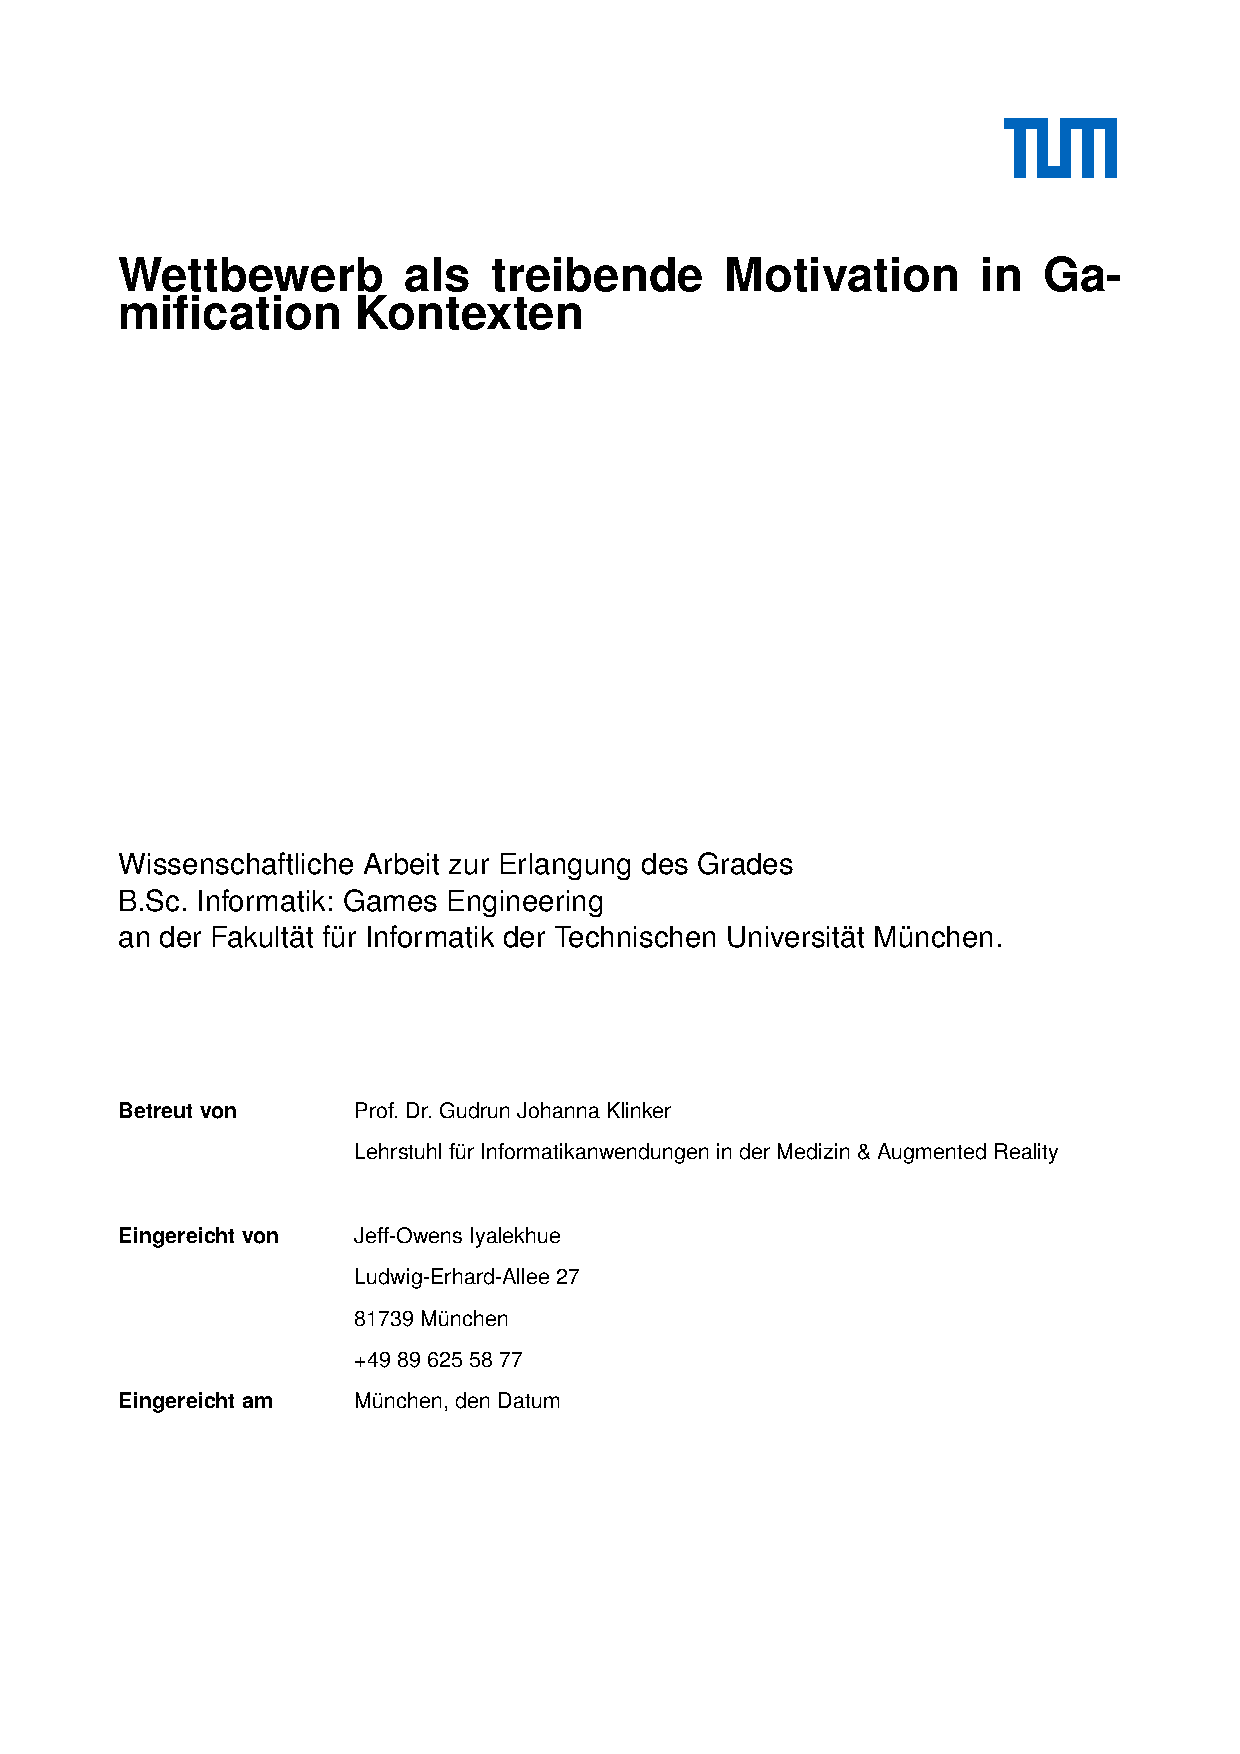
\includepdf[pages=-]{./Ressourcen/Deckblatt.pdf}
\tableofcontents % Inhaltsverzeichnis

\chapter{Kurzzusammenfassung}

\chapter{Einleitung}
\section{Motivation}
Gamification ist mittlerweile eine Methode, die häufig dafür verwendet wird um Applikationen neu zu designen mit dem Ziel, dass diese ansprechender und effektiver sind. Auch werden einige Studien zu diesem Thema durchgeführt um die Wirkungen und Einflüsse durch die Anwendung zu ergründen. Dies fokussiert sich oft in einem Anwendungsbereich, zum Beispiel es Schülern beim lernen hilft. Verschiedene Aspekte aus Spielen können angewendet werden um ein Design zu alternieren, die Facette, die in dieser Arbeit betrachtet wird ist der Wettbewerb.
Kompetitive Komponenten sind elementare Bestandteile vieler Spiele, aber auch in vielen anderen Kontexten sind sie enthalten.
In dieser Thesis wird Wettbewerb als Aspekt von Gamification Kontexten betrachtet und untersucht.
\section{Hypothesen}
\subsection{Wettbewerb beeinflusst die Leistung}
Wenn man Wettbewerb wird das eigen Handel äußeren Einflüssen ausgesetzt. So kann das Ziel eines Siegen einen motivieren oder der direkte Vergleich mit einem Gegenüber vielleicht Stress erzeugen. Daher vermuten wir, dass eine kompetitive Situation ein Individuum in seiner Leistung beeinflusst, dies kann ein förderlicher oder hinderlicher Effekt sein.
\subsection{Wettbewerb beeinflusst das empfinden der Nutzungserfahrung}
Wenn man ein und die selbe Aufgabe unter verschieden Szenarien löst, kann dies die Wahrnehmung der Handlung beeinflussen. Dies könnte sich im Empfinden einer Situation auswirken oder sich in  der Bereitschaft sich erneut in diese Situation zu begeben äußern. Wir vermuten ein kompetitiver Gedanke könnte eine Tätigkeit lohnenswerter oder abschreckender erscheinen lassen.
\subsection{Nicht-menschliche und menschliche Gegner besitzen den selben Einfluss}
Im Wettstreit vergleicht man seine Leistung mit einer anderen Leistung, daher vermuten wir ist es nicht relevant wer oder die andere Leistung erbringt. Also das es dabei nicht relevant ist ob der Gegner menschlich oder nicht-menschlich ist.

\section{Definitionen}
\subsection{Gamification}
Gamification beschreibt den Vorgang Komponenten, welche für Computerspiele charakteristisch sind, zu einer anderen Anwendung hinzu zu fügen. Dies soll der Verbesserung der modifizierten Anwendung. So soll das Interesse der Nutzer dadurch gesteigert oder ein Lerneffekt erhöht werden.\cite{deterding2011game}
\subsection{Wettbewerb und Motivation}
Wettbewerb lässt sich als das Vergleichen von Leistungen definieren und dient als extrinsische Motivation. Motivation lässt sich zwei Arten unterscheiden: intrinsiche und extrinsische Motivation.%\newline
Der intrinsische Motivation entspringt einem inneren Antrieb seine eigenen Fähigkeiten zu bestätigen.%\newline
Im Gegensatz dazu steht die extrinsische Motivation, bei der der Anreiz von einem äußeren Faktor entspringt. Im Fall eines Wettbewerb wäre der Anreiz üblicherweise der Sieg und damit das Besiegen des Gegenübers.\cite{Deci1981}

\chapter{Ansatz und Vorgehensweise}
 Um den Einfluss von Wettbewerb in der Leistung innerhalb eines spielerischen Szenarios beobachten zu können, braucht man eine Umgebung, in welcher dies unter verschiedenen Gesichtspunkten, möglich ist. Für diesen Zweck bietet sich die Implementation eines simplen Computerspiels an, mit dem die kognitiven Fähigkeiten einer Person testen, die Schwankungen in der Leistung aufzeichnen und verschiedene Testszenarien überprüfen kann. Als Spiel wird ein Mathespiel umgesetzt, in dem die Probanden Kopfrechnugnen lösen. Zudem sollen die Teilnehmer der Testgruppen einen Fragebogen ausfüllen, der die Beobachtungen der Spielsituationen in einen weiteren Kontext setzt.
 
\section{Modi und Testszenarios}
Verschiedene Szenarios in denen Wettbewerb in einer Form umgesetzt ist sind denkbar. Im Verlauf der ersten Planung  wurden Situationen festgelegt, die interessant für die das Bestätigen oder Widerlegen der aufgestellten Thesen sind. Diese Situationen sollen in Spielmodi abgebildet werden.\newline
Diese Modi sind Variationen eines Standardmodus. Dieser Ursprungsmodus lässt sich mittels der Einstellungen modifizieren. Änderungen durch veränderte Einstellungen sind zum Beispiel die Dauer des Spiels, das Anzeigen der erzielten Punkte oder der verbleibenden Zeit. Das Spiel terminiert entweder manuell nach dem betätigen der 'Escape'-Taste oder nach einer gesetzten Zeit, da diese auch als 'unendlich' eingestellt werden kann, ist das händische Beenden immer möglich. Die Aufgaben können während eines Spieldurchlaufs zufällig generiert werden oder im Vorfeld erstellt, gespeichert und dann für ein Spiel geladen werden. Im folgenden werden alle implementierten Modi beschrieben:\itemize

\item''Singleplayer''-Modus:\newline
Dieser Modus entspricht dem Basisspiel in dem keine Wettbewerbssituation vorhanden ist. Man spielt ohne Gegner und versucht einen möglichst hohe Punktzahl zu erzielen. Die Anzeige auf dem Bildschirm entsprechen der Abbildung \ref{fig:singleplayer}.
\item''Halb-Coop''-Modus:\newline{}
Der Gedanke in dieser Variante ist das zwei oder mehrere Menschen den Einzelspielermodus parallel spielen. Dadurch soll ein indirekter Wettbewerb entstehen, da die Spieler im Grunde für sich alleine spielen, aber ein Vergleich der eigenen Performanz mit einer anderen Leistung möglich ist. Dafür synchronisiert sich der Start des Spiels der Personen. Ansonsten entspricht alles dem Basisspiels. Das Erscheinungsbild entspricht dem ''Singleplayer''-Modus
\item''Versus''- \& ''Versus2''-Modus:\newline
Der ''Versus''-Modus entspricht einer klassischen Umsetzung von Wettbewerb, zwei Spieler spielen gegen einander. Die Punktzahlen von beiden werden gegenübergestellt, damit ein Vergleich der Leistung stattfinden kann. Die Punkteanzeige auf dem Bildschirm eines Nutzers ist in dieser Variante leicht modifiziert,  vergleiche Abbildung \ref{fig:versus}, denn sie zeigt  auch den Punktestand des Gegenübers an (Bsp. X vs. Y, mit X als die Punktzahl des Spielers und Y als die des Gegners). Die zwei Varianten unterscheiden sich nur im Namen, diese Unterteilung ist für die Logbuchdateien notwendig.
%\item''Versus 2''-Modus:\newline
\item''Party''-Modus:\newline
Um den Wettbewerb mit mehreren Teilnehmern darzustellen wurde dieser Modus implementiert. Die Teilnehmerzahl ist variabel und wird mit ''falschen Spielern'' von Spiel aufgefüllt, wenn eine gewünschte Spielerzahl nicht mit Nutzern erreicht wird. Das Userinterface ähnelt mehr dem der Einzelspielermodi als dem der ''Versus''-Modus, mit einem unterschied es gibt eine Ranglistenanzeige, die die Punkte der Nutzer und der, falls vorhanden, falschen Spieler in Verhältnis setzt. Die Person ganz oben in der Liste hat die höchste Punktzahl, wenn man nicht an dieser Position ist signalisiert die Liste das, indem sie leicht pulsiert. Abbildung \ref{fig:party} zeigt eine Bildschirmaufnahme dieses Modus.
\item''Collab''-Modus:\newline
Ein Modus, der etwas gegen den Gedanken der anderen Modi geht, wurde auch implementiert.  In diesem Modus kooperieren die Spieler um einen gemeinsamen Punktstand zu erhöhen. In diesem Modus entspricht der Bildschirm wieder dem des Basisspiels, der unterschied zwischen einem eigen Beitrag zum Punktestand und dem eines Mitspielers, ist die Animation ob man einen oder keinen Punkt hinzugefügt, beziehungsweise abgezogen hat. Ähnlich wie der ''Halb-Coop''-Modus entspricht die Anzeigeart der des ''Singleplayer''-Modus.

\section{Implementation}
Implementiert wird ein Spiel, das die festgelegten Testszenarios beinhaltet,  in dem mathematische Probleme mittels Kopfrechnen gelöst werden und ein Fragebogen wird erstellt, der weitere Beobachtungen festhalten soll. Die erst Implementation wird in einer Vorstudie getestet, um eine bestmögliche Version für die Hauptstudie zu entwickeln. Auch wird anhand Daten der Vorstudie ein Durchschnittsnutzer erstellt, der dann in der Hauptstudie als Gegner dienen kann.
%Die Implementation kann in drei Bestandteile untergliedert werden. Im ersten Teil wird das Spiel entwickelt, mit dem später die Studie durchgeführt werden soll. Um zu überprüfen, ob dies wie erwartet funktioniert, wird eine Vorstudie durchgeführt. Anhand der Vorstudie sollen Fehler im Spiel behoben werden und erste Ansätze für die folgenden Beobachtungen in der Studie gefunden werden. Der letzte  Teil ist schließlich die Erkenntnisse der Vorstudie umzusetzen und die Testumgebung für die Studie vorzubereiten.

\subsection{Software}
Für die Entwicklung wird die Unity Engine 2018.2.2f1 von \url{https://unity3d.com} verwendet. Diese Entwicklungsumgebung für Spiele bietet einige Grundlagen und Vorlagen, welche sich anbieten, da eine eigene Entwicklung einer Engine nicht zielführend für die Arbeit ist.  Um die Fragebögen zu erstellen wurde der Dienst ''Google Formulare'' (\url{https://www.google.com/intl/de/forms/about/}) verwendet. Für die Analyse der Daten wird Microsoft Excel(\url{https://products.office.com/de-de/excel}) verwendet.

\subsection{Spielablauf}
In diesem Abschnitt wird der Ablauf ab Beginn des Programms beschrieben. Die Oberflächen bestehen aus Knöpfen und Eingabefeldern, navigiert und interagiert wird mittels Maus und Tastatur. Der erste Bildschirm ist das Netzwerkmenü (Abbildung \ref{network}), in welchen man wählen kann ob man als Host spielen will oder als Client. Für den Fall, dass man als Client spielt kann man in die Netzwerkadresse des Hosts und den dazugehörigen Port ändern.\newline
Nach der Wahl zu hosten oder nicht wird man in das Hauptmenü (Abbildung \ref{fig:menuhost} und \ref{fig:menuclient}) weitergeleitet. Von hier aus kann man eine Runde des Spiels starten, wenn man Host ist, besitzt man die Berechtigung den Spielmodus zu wechseln(Abbildung \ref{fig:menumodi}). Auch kann man in die Einstellungen wechseln, sich vom Netzwerk trennen und damit zurück in das Netzwerkmenü und die Software beenden.\newline
In den Einstellungen kann man den Pfad angeben auf dem die Daten gespeichert werden sollen. Unter diesem Pfad werden die Logbuchdateien einer Spielrunde gespeichert, sowie die generierten Aufgaben. Wenn man Aufgaben erstellen will kann man hier sagen wie viele Funktionen pro Runde generiert werden sollen. Alternativ kann man auch einstellen, dass die Aufgaben während des Spielens zufällig erzeugt werden. Weitere Einstellungen beziehen sich auf die Darstellung des Spiels. So ist es möglich die Anzeigen für die verbleibende Zeit und die Punkte jeweils zu deaktivieren. Die Dauer einer Spielrunde wird auch hier bestimmt man kann, also angeben ob eine Runde nach einer gewünschten Zeit endet oder solange weiter geht bis der Nutzer sie per Tastendruck beendet. Auch die Lautstärke der Musik und der Soundeffekte lassen sich in den Einstellungen regulieren. Informationen zu dem Spieler die für die Logbuchdateien benötigt werden, werden auch hier angegeben, dazu zählt die Identifikationsnummer und das Geschlecht. Auch die Angabe in wie viele Runden bereits gespielt wurden lassen sich hier verändern. Wenn man die Einstellungen werden diese gespeichert, nur die Informationen zu einen Nutzer werden nicht persistent hinterlegt.

Im Hauptmenü kann eine Spielpartie gestartet werden in dem auf den  ''Start''-Knopf gedrückt wird und alle nötigen Teilnehmer für den Modus bereit sind. Der ''Singleplayer''-Modus kann immer sofort starten, die anderen Modi verzögern den Spielstart bis alle mit dem Host verbundenen Spieler mit dem ''Start''-Knopf ihre Bereitschaft signalisiert haben. Während der Verzögerung können Nutzer durch erneutes betätigen des Knopfes die Bereitschaft wieder aufheben.\newline
Im Spiel hat man mehrere Anzeigen und ein Eingabefeld. Die folgende Oberfläche beschreibt einen generellen Fall des Spielmodus und trifft am ehesten auf den ''Singleplayer''-Modus zu. Die Anzeige am mittigen, oberen Bildschirmrand ist die verbleibende Zeit, darunter findet man die ''Score''-Einblendung. Zentral und im Verhältnis am größten dargestellt findet man die zu lösende Rechnung. Unterhalb der Aufgabe ist das Eingabefeld in dem die Lösung eingegeben wird. Zur Eingabe wird die Tastatur verwendet, wobei nur Zahlen eingeben und das '-'-Zeichen akzeptiert werden. Mit der ''Enter/Return''-Taste wird eine Eingabe bestätigt, mit der ''Backspace''-Taste können unbestätigte Eingaben wieder rückgängig gemacht werden. Wenn eine Aufgabe richtig beantwortet bekommt man einen Punkt zum Score hinzu, dies wird durch einen Ton und einer Animation zusätzlich visualisiert. Für den Fall einer falschen Lösung wird die Punktzahl um einen Punkt reduziert, dass überspringen einer Aufgabe ist auch möglich wenn eine leere Eingabe bestätigt wird. Überspringen gibt keinen Punkt zum Score, zieht aber auch keinen ab. Auch das Verlieren oder überspringen einer Aufgabe hat jeweils eine eignen Animation und einen Ton.\newline
Wenn man in den Einstellungen gewählt hat das man ''Supervisor'' ist hat man eine abgewandelte Variante der Modi, die änderungen sind in allen Modi gleich. Mit diesen Einstellungen muss muss kann man die Rechnungen nicht mehr selbst beantworten, denn die Aufgaben werden von einem Skript selbstständig richtig gelöst. Nach einer bestimmten Zeit wird die Lösung eingegeben und bestätigt. Bis zur Bestätigung wird im Eingabefeld die verbleibende Zeit bis dahin und etwas unterhalb des Feldes die korrekte Lösung angezeigt. Beide Anzeigen sind so Platziert, dass sie eher schwer zu erkennen sind, wenn man nicht von ihnen weiß. Zusätzlich ist es einem möglich, in dem Zeitraum bis zur autonomen Beantwortung ,die richtige Antwort zeichenweise im Eingabefeld sichtbar zu machen, in dem eine Beliebige Taste gedrückt wird. Der Zweck dieser Funktion soll es sein eine Eingabe durch den Betreuer, trotz der selbständigen Beantworten der Aufgaben vor zu täuschen.  Die Zeitspanne zwischen den Antworten ist anfangs anhand gegebener Werte festgelegt, wenn es einen Gegner gibt, ändert sich dynamisch. Denn sie ist das Mittel der letzten drei Abständen in denen der Gegenüber eine Aufgabe gelöst hat.

\subsection{Datensammlung und Spielverlaufslogbuch}
Während eines Spieldurchlaufs wollen wir verschiedene Faktoren beobachten, um Rückschlüsse auf die Einflüsse der Testszenarien  machen zu können. Für diesen Zweck sammeln wir  Daten des Spielverlaufs und lassen sie uns für eine spätere Analyse speichern. Vom Spiel werden nach einer Runde drei Dateien angelegt, die die gewünschten Ereignisse dokumentieren. Die Logbuchdateien eines Spielers werden in einen Ordner unter einem angegeben Pfad gespeichert, welcher in der Form ''ParticipantX'', wobei X der jeweiligen Nutzeridentifikationsnummer entspricht (Bsp. Participant1), benannt wird. Die drei Dateien einer Runde Unterscheiden sich im Dateiformat und gering  im Informationsgehalt. Die im Spiel zu beobachteten Variablen werden zum einen serialisiert und dann als ''.dat'' gespeichert, diese Dateien dienen ausschließlich als redundante Sicherheitskopie und könnten wieder deserialisiert und  geladen werden. Dies ist im Code nicht umgesetzt worden, da keine Notwendigkeit bestand.\newline
Um den Verlauf einer Runde in der Retrospektive nachvollziehen zu können, werden als ''.txt''-Dateien stichpunktartige Protokolle der Ereignisse dokumentiert. Im Ersten Part der Textdatei findet man ein Resümee der Endwerte, gefolgt von einer Beschreibung des Lösungsvorgangs einer Aufgabe.\newline
Für die Datenauswertung  werden hauptsächlich die ''.csv''-Dateien verwendet. Solche Dateien können in Programmen, die speziell für die Datenverarbeitung  und Analyse dienen, eingelesen und verarbeitet werden. Die Daten ein Jeder Aufgabe einer Runde Werden tabellarisch hinterlegt, damit sie später in Excel eingelesen werden und ausgewertet können.
 
\subsection{Quellcode Zusammenfassung}
Die verwendete Programmiersprache ist C\#. In der Verwendung mit der Unity Engine wird auch dazugehörige Namespaces verwendet die wichtige Klassen und Funktionen zum erstellen eines Spiels anbieten (\url{https://docs.unity3d.com/ScriptReference/}). Dazu gehört die Klasse MonoBehviour, von der einige Klassen erben um in der Spielschleife eingebunden zu sein. Diese Skripten müssen einem GameObject im Editor zu gewiesen werden. Wenn ein Klasse zu greifen UnityNetworking  soll, muss sie von NetworkBehavior erben anstatt von MonoBehaviour. Die wichtigsten, selbst erstellten C\#-Skripten werden im folgenden zusammengefasst und ihr Nutzen beschrieben.

\subsubsection{GameManager.cs}
Diese Klasse verwaltet die Einstellungen mit den dazugehörigen Variablen. Diese Klasse ist als Singleton angelegt. Dies bedeutet es existiert immer eine Instanz dieser Klasse und es kann aber auch nie mehr als eine geben. Dieses Objekt kann von allen anderen Skripten referenziert werden, daher beinhaltet diese Klasse Variablen, die den Status des Spiels beschreiben, wie zum Beispiel der aktuell gewählte Spielmodus. Zudem werden in der Datei die Helferklassen ParticipantData, TaskData, GeneratedTasks und OptionsData deklariert, diese werden für die Strukturierung und zum persistenten Speichern der Informationen benötigt. So bietet GameManager je eine Funktion die Variabeln der Einstellungen zu sichern und zu laden. 
Eine andere Funktion die diese Klasse bietet, ist das vorab generieren von Aufgaben für eine Spielrunde. Die von GerenateTask() erstellten Aufgaben können mittels LoadGeneratedTasks() geladen werden und so dann in GameLogic.cs verwendet werden.
Ein weiterer Dienst, der hier gestellt wird, ist CreateUserData(ParticipantData participant). Hier mit werden Dateien angelegt die als Logbuch einer Spielrunde dienen.

\subsubsection{GameLogic.cs}
Diese Klasse beinhaltet die Logik des Mathespiels. Zu Beginn wird die Coroutine StartCountdown() aufgerufen um den Start der Hauptschleife in der Update Funktion mit einem Countdown  zu verzögern. In der Game-Loop wird überprüft, ob eine Kondition zum Beenden der Spielrunde erfüllt wird. Hier für wird überprüft ob es eine Eingabe der ''Escape''-Taste gab oder die Spielzeit abgelaufen ist. Beim beenden der Runde wird, mit Hilfe der Instanz der GameManager-Kasse,die Runde in definierten Logbuch-Dateien protokolliert, ein Endbildschirm angezeigt und das Hauptmenü geladen. Zudem wird in dieser Schleife die Hilfe für einen Spieler der als ''supervisor'' in den Einstellungen gesetzt wurde abgehandelt. Dazu gehört der Countdown der anzeigt wann die aktuelle Aufgabe autonom gelöst wird, das Lösen der Aktuellen Aufgabe und das schrittweise füllens des Eingabefelds mit der Lösung. Wenn allgemein eine Aufgabe gelöst wurde wird die Task()-Funktion aufgerufen. Diese Methode erstellt oder lädt die nächste Aufgabe.\par
Mit der Solve()-Funktion wird die Antwort im Eingabefeld bestätigt, geprüft und dem entsprechend reagiert. So werden leere Eingaben  mit null Punkten, falsche mit minus einem und richtige mit plus einem Punkt zu dem aktuellen Punktenstand vergütet. Auch werden die Informationen über den Verlauf der Beantwortung der Aufgabe als TaskData-Objekt in einer Liste eingefügt.

\subsubsection{MenuScript.cs}
Hier werden die Funktionen des Menüs zur Verfügung gestellt. Einige Funktionen dienen allein dafür in den Einstellungen die Variablen des GameManager zu ändern oder auf dessen Funktionen zu zugreifen. Diese Funktionen werden dann im Editor UI-Knöpfen oder  UI-Reglern zugewiesen, sodass sie in der Anwendung eingestellt werden können.

\subsubsection{NetworkMenu.cs}
Hiermit wird die Netzwerkverbindung erstellt, verwaltet oder getrennt. Um in der Lage zu sein darauf zugreifen zu können hat er den NetworkManger referneziert, dies ermöglicht es einen Host oder Client zu erstellen und die Verbindungsinformationen anzupassen. verschiedene Funktionen wie PlayAsHost() realisieren dies. Mittels setPort(string port) lässt sich die Portnummer und mit SetNetworksddress(string ip) die Netzwerkadresse des Servers eingeben.

\subsubsection{NetworkSync.cs}
Eine Helferklasse, als Singleton designt ist, mit der die Abläufe einer Netzwerkverbindung synchronisiert werden sollen. 
Auch  erstellt und  verwirft sie NetworkObject-Objekte mittels einer Coroutine für Spielrunden in denen weitere Spieler durch falsche simuliert werden sollen.

\subsubsection{NetworkObject.cs}
Die Repräsentation eines Clients im Spiel. Auch können hier mit falsche Spieler emuliert werden. Das GameObject, dass dieses Skript zugewiesen hat, muss auch die  Komponente NetworkIdenty besitzen. Dies ist notwendig damit das Objekt eine eigene Identät im Netzwerk besitzt, wenn es sogar den Client des eigen Spiels repräsentiert, besitzt es lokale Autorität. Mit der connectionID identifiziert er sich in in einem Spielsitzung. Die Hauptaufgabe dieses Skirpts ist dem Server Änderungen des Clients, wie zum Beispiel eine neue Punktzahl, mitzuteilen. Wenn ein Spieler imitiert werden soll, wird das Verhalten für diesen auch hier erzeugt.

%\subsection{Vorstudie}
%Mit der Vorstudie wurde die Lauffähigkeit des Spiels getestet und versucht einen ersten Ansatz für mögliche Beobachtungen in der Haupttestreihe zu finden. Es wurden die Modi ''Singlepayer'', ''Halb-Coop'', ''Versus'' und '' Party'' von fünf Teilnehmern gespielt. Anhand der Impressionen wurden Fehler im Spiel ausgebessert und Änderungen vorgenommen, so wurden die Eingangs- und Austrittsanimationen der Aufgaben entfernt damit ein ununterbrochener Spielablauf entstehen kann. Auch die Wahl der zu testenden Modi wurde geändert. Die nun in der Hauptstudie zu Testenden Szenarien sind  ''Singleplayer'', ''Halb-Coop'', ''Versus'' und ''Versus2''.

\subsection{Fragebogen}
Neben der reinen Beobachtung des Spielverlaufs sind auch Ausagen und Eindrücke der Spieler nützlich um Daten in Kontexte zu stellen und zu Interpretieren. Hierfür eignet sich die Beantwortung eines Fragebogens durch die Teilnehmer. Der Fragebogen lässt sich in drei Abschnitte aufteilen, der erste Part ist zu beginn, also vor dem ersten Spielen, zu beantworten, gefolgt von Abschnitten die sich mit dem Spielen eines Modus abwechseln und endet mit einem Teil als Resümee.
\subsubsection{Prä-Spiel }
Hier wird der Teilnehmer befragt wie er seine Fähigkeit der Kopfrechnungen durchzuführen einschätzt, dies kann man später in Relation mit dem Erfolgserlebnissen setzten. Um Diese Fest zu stellen wird der Gefühlzustand auch in diesem Abschnitt abgefragt,um einen Nullwert für die vergleiche zu besitzen. Die Gefühlslage soll vom Spieler insofern angegeben werden ob er sich zu dem Zeitpunkt des Beantwortens gestresst oder erleichtert fühlt. Auch wie die Nutzer zu Wettbewerb in verschiedenen Kontexten sehen wird gefragt.
\subsubsection{Spiel}
Dieser Abschnitt wiederholt sich vier Mal, da diese Fragen nach jeder Runde, die gespielt wurde, zu dem jeweiligen Modus gestellt werden. Dazu gehört  wie der Modus gefallen hat, wie die Zeitdauer war, ob der Modus erneut gespielt werden würde und die Gefühlslage soll angegeben werden.
\subsubsection{Post-Spiel}
Zum Schluss soll bewertet werden wie das Spiel im Gesamten gefallen hat und die Modi sollen untereinander eingestuft werden, auch soll erneut angegeben werden welche Modi erneut gespielt werden würden.

\section{Aufbau}\label{sec:Aufbau}
Für einen Durchlauf wird ein einzelner Teilnehmer in den Versuchsaufbau gebeten. Es sind zwei Computer aufgebaut auf denen das Spiel läuft und die über das Netzwerk miteinander verbunden sind. Zunächst füllt der Proband den ersten Teil des Fragebogen aus. Anschließend spielt er einen Modus und beantwortet danach den zugehörigen Teil des Fragebogens. Dies wiederholt er bis er alle Modi gespielt hat. Die Reihenfolge der Modi für jeden Teilnehmer durch, sodass erst bei mehr als 24 Teilnehmern die Reihenfolge sich wiederholt. Die verschiedenen Spielszenarien haben unterschiedliche Aufbauten, die alle gemein haben, dass der Proband einen Bildschirm zur Wiedergabe des Spiels und Maus und Tastatur zur Eingabe vor sich hat. In der Einzelspielervariante ist dies bereits die gesamte Aufstellung und der Betreuer dient ausschließlich als Aufsicht. Ausschließlich der ''Singleplayer''-Modus nutzt diesen Aufbau. Die nächste Konstellation ist für alle Modi die mehr als einen Spieler benötigen. besitzt jeder seinen eigenen Grundaufbau, dieser ist von den anderen Spieler nicht einsehbar. Der Betreuer kann hierbei auch ein Mitspieler sein, in diesem Fall kann er die Bildschirme der anderen einsehen. Der ''Halb-Coop''-Modus hat einen leicht abgewandelten Aufbau, den die Bildschirme sollen hier für die Gegenspieler sichtbar sein. Da es Organisatorisch leichter abzustimmen ist, werden die alle Modi mit maximal zwei echten Spielern gespielt. Der Opponent wird in jeden Fall die Versuchsleitung sein, somit ist der Gegner eine Konstante in der Studie. Da die Versuchsleitung alles Begutachten muss, darf sie die das Spiel und die Eingabe des Spielers einsehen. Im ''Halb-Coop''-Aufbau wird das Spiel der Aufsicht mittels eines zweiten Bildschirms für den Probanden sichtbar. Nach dem vier Modi gespielt wurden muss der Teilnehmer den letzten Abschnitt des Fragebogens ausfüllen.

%Zwischen den Spielszenarien lassen sich drei verschieden Aufbauten definieren, die alle die gemein haben, dass die Versuchsperson nicht alleine sondern immer unter Aufsicht des Betreuers ist. Beim ''Singleplayer''-Modus spielt der  Teilnehmer alleine und wird vom Versuchsleiter nur beobachtet. Der ''Halb-Coop''-Modus  versucht einen indirekten Wettbewerb aufzubauen in dem der Spieler zeitgleich mit dem Betreuer den ''Singleplayer''-Modus spielt und zusätzlich die Möglichkeit bekommt den Bildschirm des Gegenübers zu sehen. Allerdings wird ihm dieses Szenario als eine Variante beschrieben wo er nur auf sein Spiel achten braucht. Im Gegensatz dazu wird in den Modi ''Versus'' und ''Versus2'' direkt auf den Vergleich der Punktzahlen hingewiesen. In diesen Varianten sieht der Spieler nur seinen eigenen Bildschirm und bekommt daher nur über den Anzeigen in seinem Spiel den Fortschritt seines Gegenspieler mit. Der Unterschied der beiden Szenarien ist die narrative die man dem Teilnehmer liefert, im ''Versus''-Modus wir ihnen erzählt, dass sie gegen die Person spielen, die sie beaufsichtigt. Im '' Versus2'' spielen sie angeblich gegen einen künstlichen  Gegner, der anhand des durchschnittlichen Spielers, der sich aus der Vorstudie ermitteln lies, generiert wurde. Faktisch spielt der Versuchsleiter zu keinen Zeitpunkt mit oder gegen die Teilnehmer, jedes mal wenn ein zweiter Spieler benötigt wird, spielt sie gegen die selbe Instanz. Der Gegenspieler ist ein simpler Algorithmus, der anhand der letzten drei Antwortzeiten des Teilnehmers seine eigene eigene errechnet.%anpassen!!!
\subsection{Beobachtungsgruppen}
Für die Untersuchung wurden keine speziellen Kriterien für die Wahl der Teilnehmer im vor hinein gefällt, denn organisatorisch ist im gegebenen Rahmen eine breit differenzierte Teilnehmerauswahl problematisch. Daher werden Gesichtspunkte wie zum Beispiel Altersgruppen, Geschlecht und Bildungsniveau, in der Datenauswertung nicht beachtet. Die Probanden werden versucht über direktes Ansprechen von möglichen Teilnehmern  und über Plakate versucht zu an zu werben. Angestrebt werden insgesamt um die 30 Nutzer, diese würden sich in eine kleine Gruppe für eine Vorstudie und eine Gruppe mit circa 24 Teilnehmern für die Hauptstudie aufteilen. Die Zahl 24 ergibt sich durch das Permutieren der Reihenfolge der vier Testszenarien.

\chapter{Vorstudie}
Das Ziel der Vorstudie ist mögliche Fehler im Spiel und dem Testverlauf ausfindig zu machen und erste Eindrücke zu sammeln aus denen für die Hauptreihe gelernt werden kann. Außerdem soll anhand der gewonnen Daten ein Durchschnittsspieler erfasst werden, der dann als programmierter Gegner in der Hauptstudie dienen soll.
\section{Planung}
Die Vorstudie soll im deutlich kleineren Rahmen als die Hauptstudie stattfinden um den Aufwand zu reduzieren. Die Testumgebung soll allerdings im besten Fall, der der Finalen  entsprechen. Es sollen vier bis sechs Teilnehmer das Spiel spielen und den Fragebogen ausfüllen. Getestet werden 4 Modi der ''Singleplayer'', ''Halb-Coop'', ''Versus'' und ''Party''. Jeder Spieler spielt die Modi in einer anderen Reihenfolge. Die Testumgebung ist wie in Abschnitt \ref{sec:Aufbau} beschrieben. Der ''Party''-Modus wird für vier Spieler ausgelegt, dass heißt zwei Spieler sind falsche Spieler, die durch das Spiel erzeugt werden. Dies wird dem Studienteilnehmer auch vermittelt, allerdings kann er im Spiel nicht zwischen den künstlichen und dem menschlichen Gegner unterscheiden.
\section{Evaluation}
\subsection{Teilnehmer}
%Es wurden im totalen 25 Teilnehmer rekrutiert, davon bilden 20 die Hauptgruppe. Alle Teilnehmer lassen sich in die Altersgruppe 18- 29 ein ordnen und hatten ungefähr den selben Bildungsstand, überwiegend Studierende der Mathematik oder Informatik. Die Mehrheit der Teilnehmer ist männlich.
Es wurden fünf Teilnehmer für die Versuchsreihe akquiriert. Alle Teilnehmer waren  in der Altersgruppe 18-29. Alle Probanden studieren, mit einer Ausnahme die eine abgeschlossen Berufsausbildung nachweisen kann. Die Geschlechteraufteilung ist nicht ausgewogen.
\subsection{Ergebnisse und Ablauf}
Wie zu erwarten gab es hin und wieder Probleme mit dem Programm. Sobald ein Fehler im Ablauf aufgetreten ist, wurde die Runde abgebrochen und neu gestartet. Gegebenenfalls wurde dies wiederholt bis eine fehlerfreie Runde gespielt werden konnte. Die Bugs wurden notiert und schnellst möglich behoben.\newline
Bei der Befragung ob sie Wettbewerb als hinderlich oder förderlich empfinden, sagten die Teilnehmer, dass es eher förderlich sein kann, dies am ehesten in sportlichen Kontexten. Diese Aussage lassen die Vermutung aufkommen, dass Wettbewerb einen positiven Einfluss haben könnte, wenn nicht in der Ausübung zumindest in der Empfindung einer Situation.%Die lineare Korrelation der Aussage mit der erzielten gesamt Punktzahl der Probanden ist nicht vollständig, aber größer als null.

Die Teilnehmer wurden nach jeder Runde gefragt, ob sie sich gestresst oder erleichtert fühlen. Die Probanden haben sich im Mittel tendenzielle eher erleichtert gefühlt. Als Nullwert für die Vergleiche dienen unter den Runden dient die erste Runde. Mit der Annahme, dass sich die Gefühlslage nicht zwischen den Runden verändert, wurden T-Tests durchgeführt. Die Ergebnisse widerlegen die Nullhypothese nicht. Auch korrelieren die Werte eher weniger bis auf die dritte Runde, diese steht aber auch nicht in vollständiger lineare Korrelation zur ersten Runde.

Die folgenden Auswertungen richten sich nach dem Mittelwert der Antworten aller Spieler.
Der ''Singleplayer''-Modus wurde mit einer eher guten mittleren Bewertung eingestuft. Die Nutzer fühlten sich eher erleichtert. Die Spieldauer wurde als eher kurz empfunden.
Der ''Halb-Coop''-Modus  wurde als eher mittelmäßig bewertet. Nach beenden der Runde waren die Probanden eher erleichtert. Wie im ersten betrachteten Modus wurde, die Zeit als eher kurz betrachtet.
Die Bewertung des ''Versus''-Modus waren höher als die der zuvor gegangenen Modi, er wurde als her gut bis gut gesehen.  Auch fühlten sich die Teilnehmer erleichtert nach dem Spielen. Die Zeit wurde kürzer als in dem Einzelspielermodi empfunden.
Der ''Party''-Modus wurde 
%Einfluss Leistung -> t-Test für modi und runden
%Nutzungserfahrung


\chapter{Hauptstudie}
%Endscore<->Runde --> Lerneffekt nach T-Test bestätigt
%kopfrechenskill einschätzung <-> endscores
%einstellung zu wettbewerb <-> endscores
%stimmung <-> sieg/niederlage
%stimmung <-> wahrnehmung des spiels
%sieg/niederlage <-> wahrnehmung des spiels
%wiederspielwert Modi
%Bewertung Modi --> Nach allen Runden: Versus am besten bewertet
%wiederspielwert Spiel 16/20
\section{Anpassungen}
Im Spiel gefundene Fehler werden behoben. Zudem werden die Eingang- und Austrittsanimationen für die Aufgaben herausgenommen, da diese den flüssigen Spielablauf gestört haben. Durch diese Änderung könne die Spielerdaten nicht für die Erzeugung eines Durchschnittsspieler genutzt werden. Als Ersatz wird eine der künstliche Gegner für die Hauptstudie  eine ''Sliding Window''-Methode verwenden, um die Zeiten zu generieren in der er agiert. Der artifizielle Spieler antwortet immer in Mittel der letzten drei Zeiten, in denen sein Gegner Aufgaben gelöst hat. Für die Anfangszeiten werden die Durschnittszeiten der Vorstudienteilnehmer verwendet. Dieser Spieler wird nun immer anstelle des Betreuers spielen, um den Gegner als eine Konstante in den Szenarios zu setzen. Auch werden andere Modi nun in der Hauptstudie verwendet. Der ''Party''-Modus wird durch ''Versus 2'' getauscht, da sich dieser direkter mit ''Versus'' vergleichen lässt. Außerdem wurde das Laden des Menübildschirms am Ende einer Runde verzögert, damit man seinen finale Punktzahl besser wahrnehmen kann und gegebenenfalls mit der des Gegners vergleichen kann. Eine erneute Vorstudie lies sich organisatorisch nicht vereinbaren, sodass der angepasste Versuchsaufbau direkt in der Hauptstudie genutzt wird.\newline Weitere Anpassungen zur Verbesserung des Versuchsablaufs wurden durchgeführt, wie das Umstellen der Ordnerstruktur der Logbuchdateien. Im Fragebogen wird im ersten Abschnitt bereits die Gefühlslage abgefragt, damit ein Wert vor der ersten Spielrunde vorhanden ist. Auch wurde eine Spieldemo als Video Angefügt, sodass anhand dieser das Spiel besser erklärt werden kann. Zudem werden die Fragen ins Englische übersetzt und eine leichte Änderung der Darstellungsform wurde vorgenommen, dies hatte aber keine weiteren inhaltlichen Änderungen zu folge.
\section{Evaluation}
\subsection{Teilnehmer}
20 Personen nahmen an der Hauptstudie teil, die gewünschten 24 Teilnehmer konnten nicht in der Laufzeit geworben werden. Die Probanden waren zwischen 18 und 29 Jahren alt. Das Bildungsniveau unter den Teilnehmern war vergleichbar, alle waren Studenten. Auch in der Hauptstudie war die Verteilung der Geschlechter der Teilnehmer stark einseitig.
\subsection{Ergebnisse}


\chapter{Diskussion}
\chapter{Ausblick}

% Bilder
\begin{figure}[b]
	\centering	
	\begin{subfigure}[a]{0.3\linewidth}
		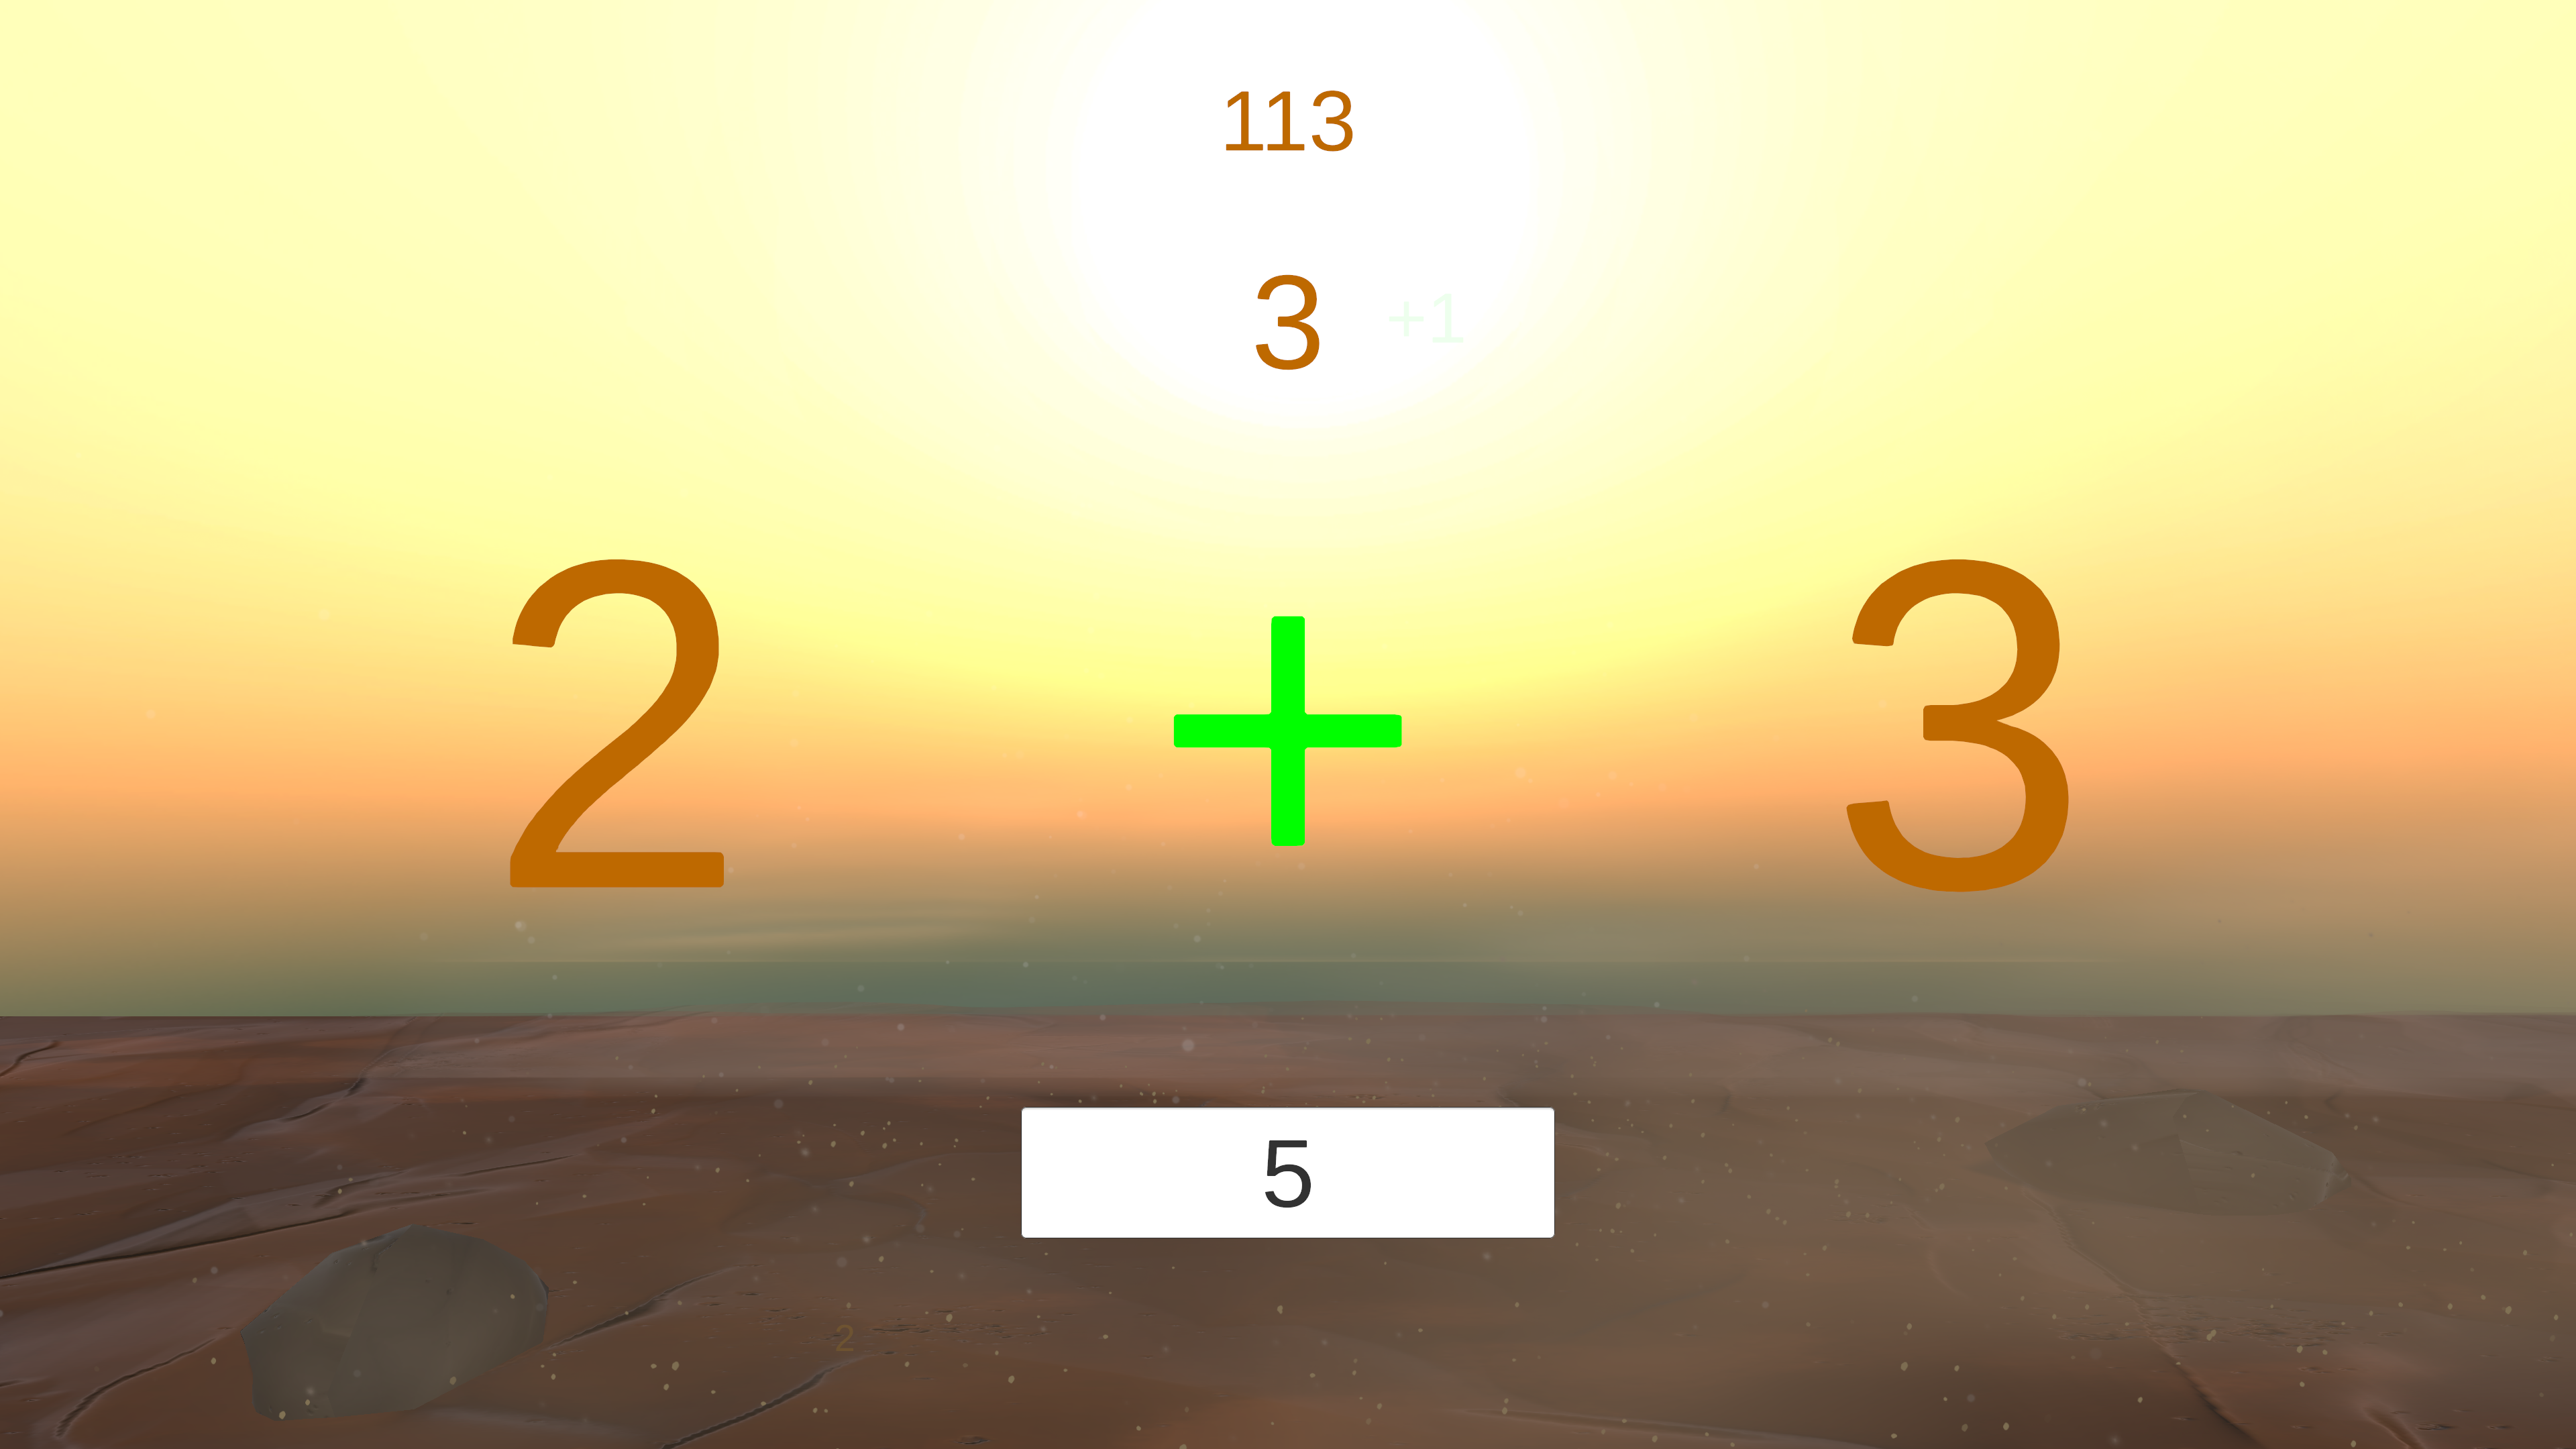
\includegraphics[width=(\linewidth)]{singleplayer}
		\caption{Singleplayer}
		\label{fig:singleplayer}
	\end{subfigure}	
	\begin{subfigure}[a]{0.3\linewidth}
		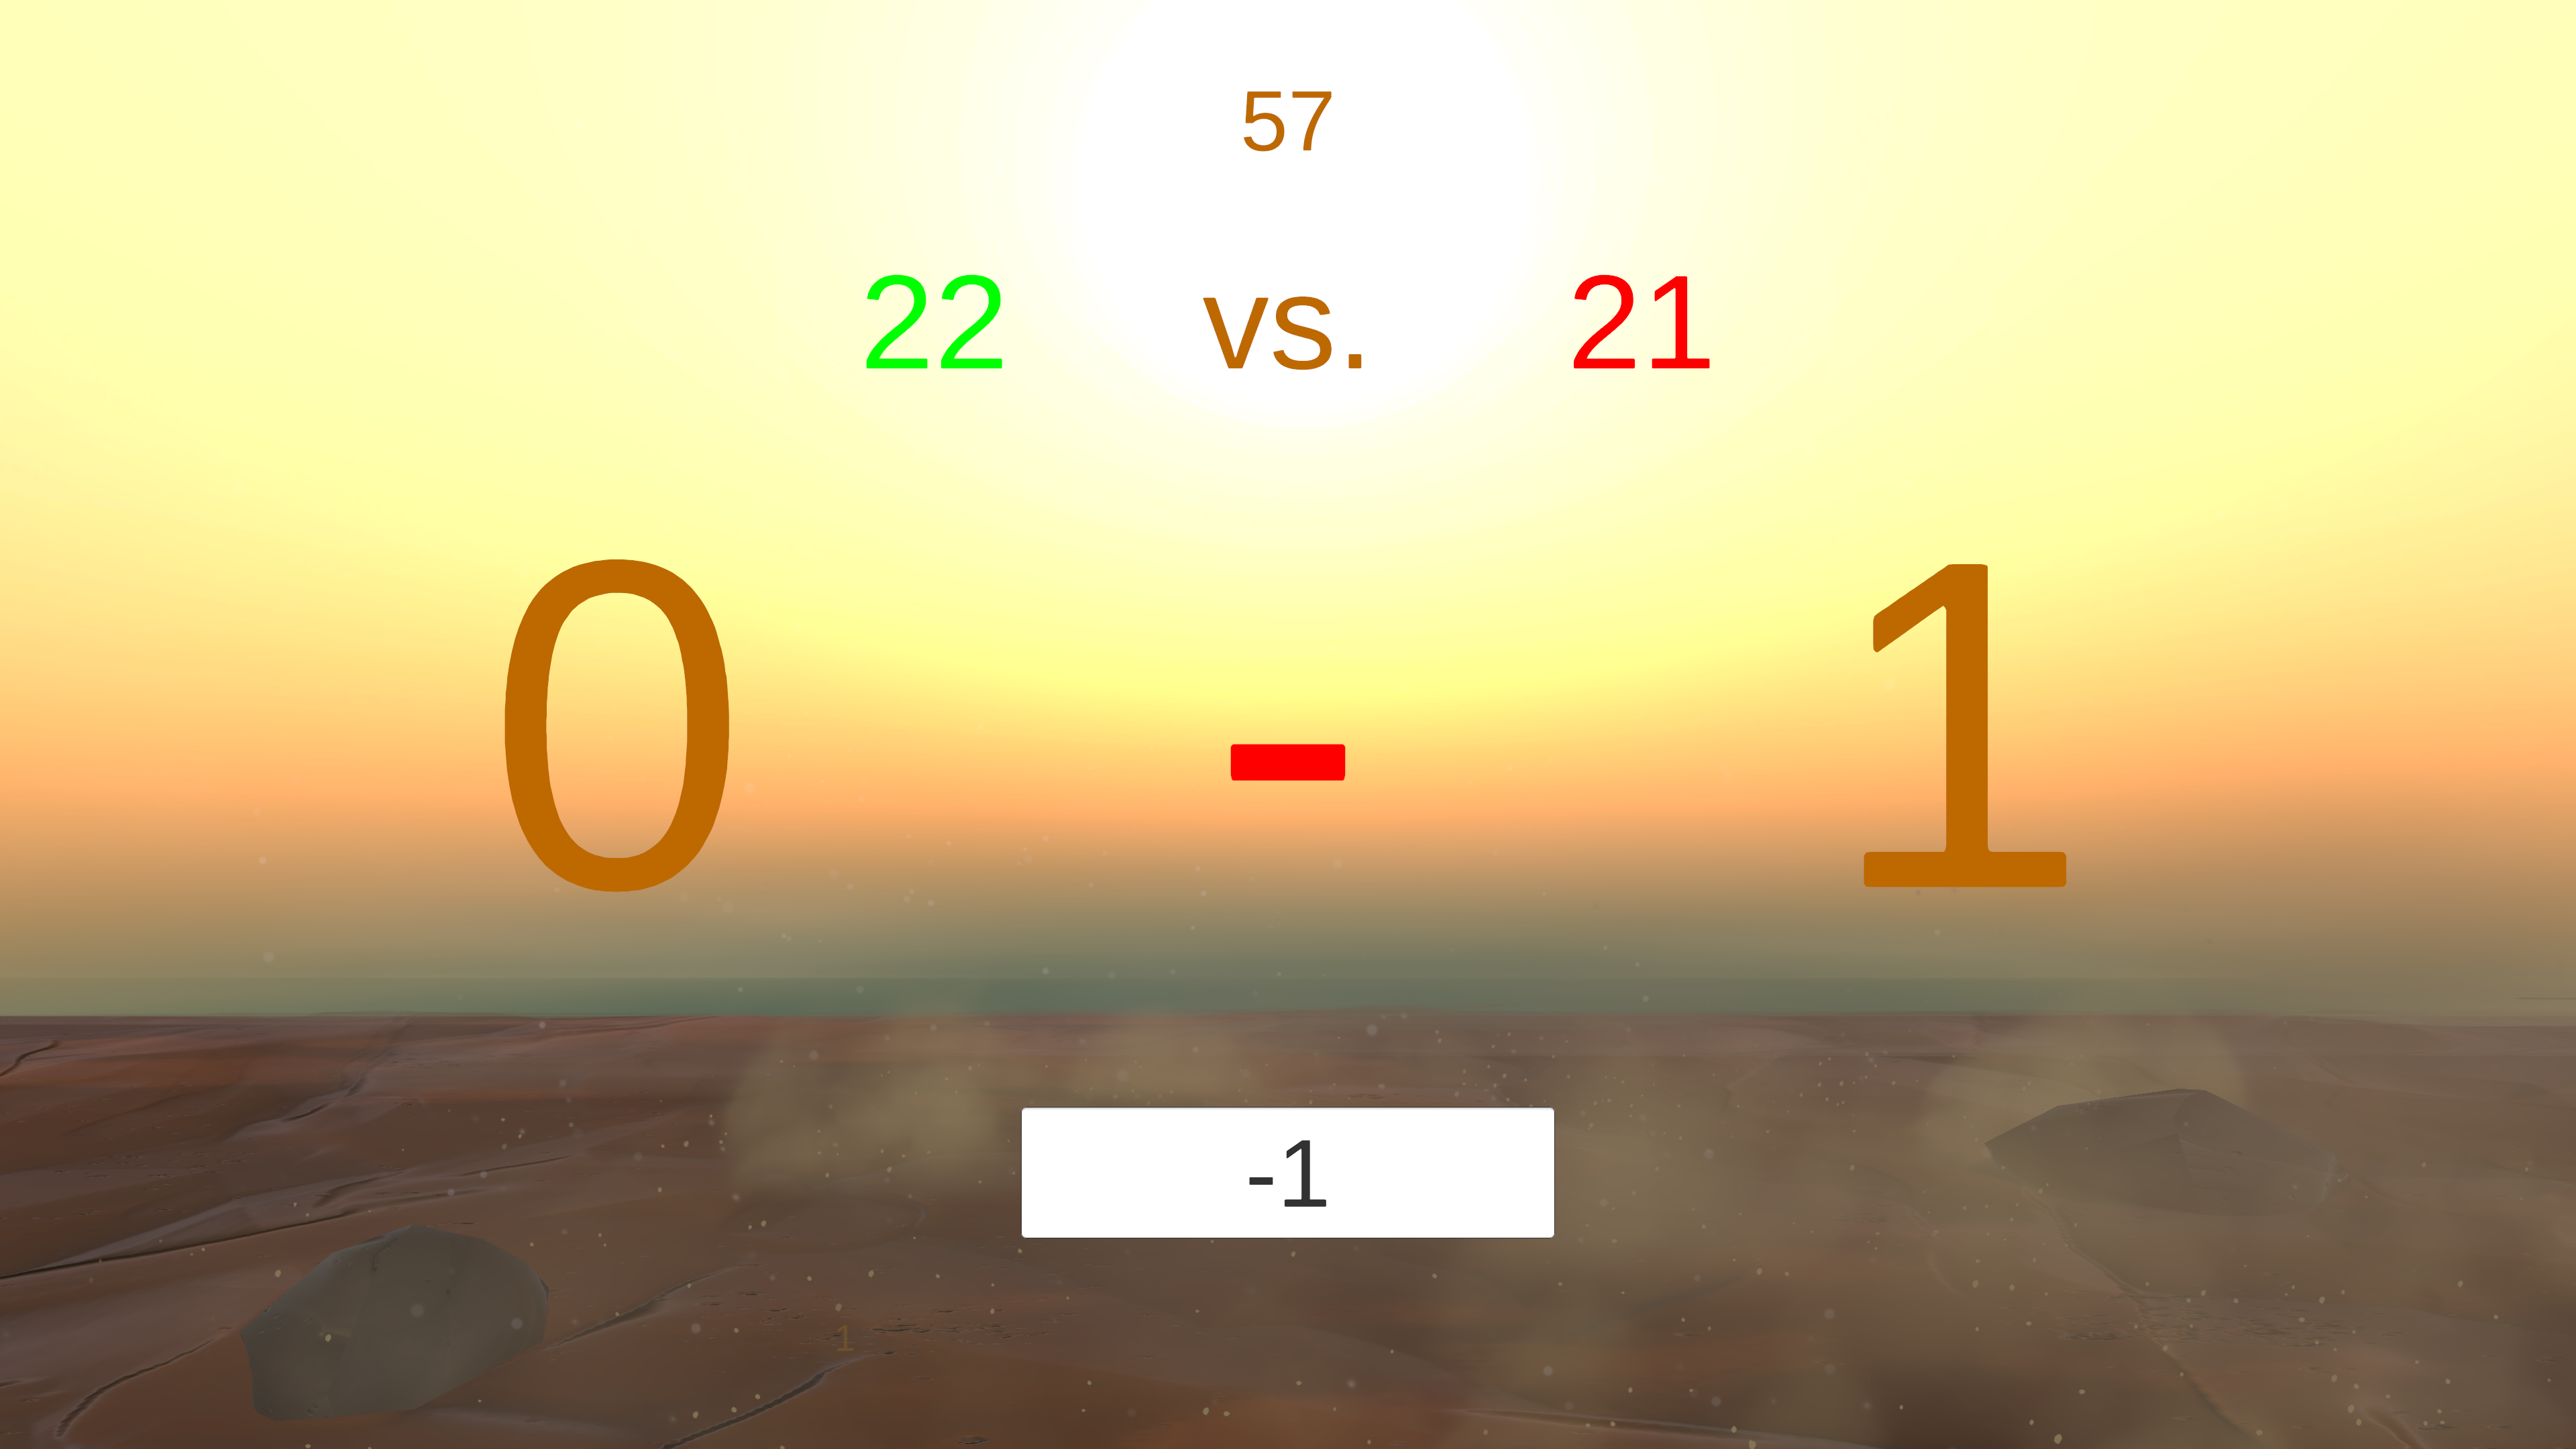
\includegraphics[width=(\linewidth)]{versus}
		\caption{Versus}
		\label{fig:versus}
	\end{subfigure}
	\begin{subfigure}[a]{0.3\linewidth}
		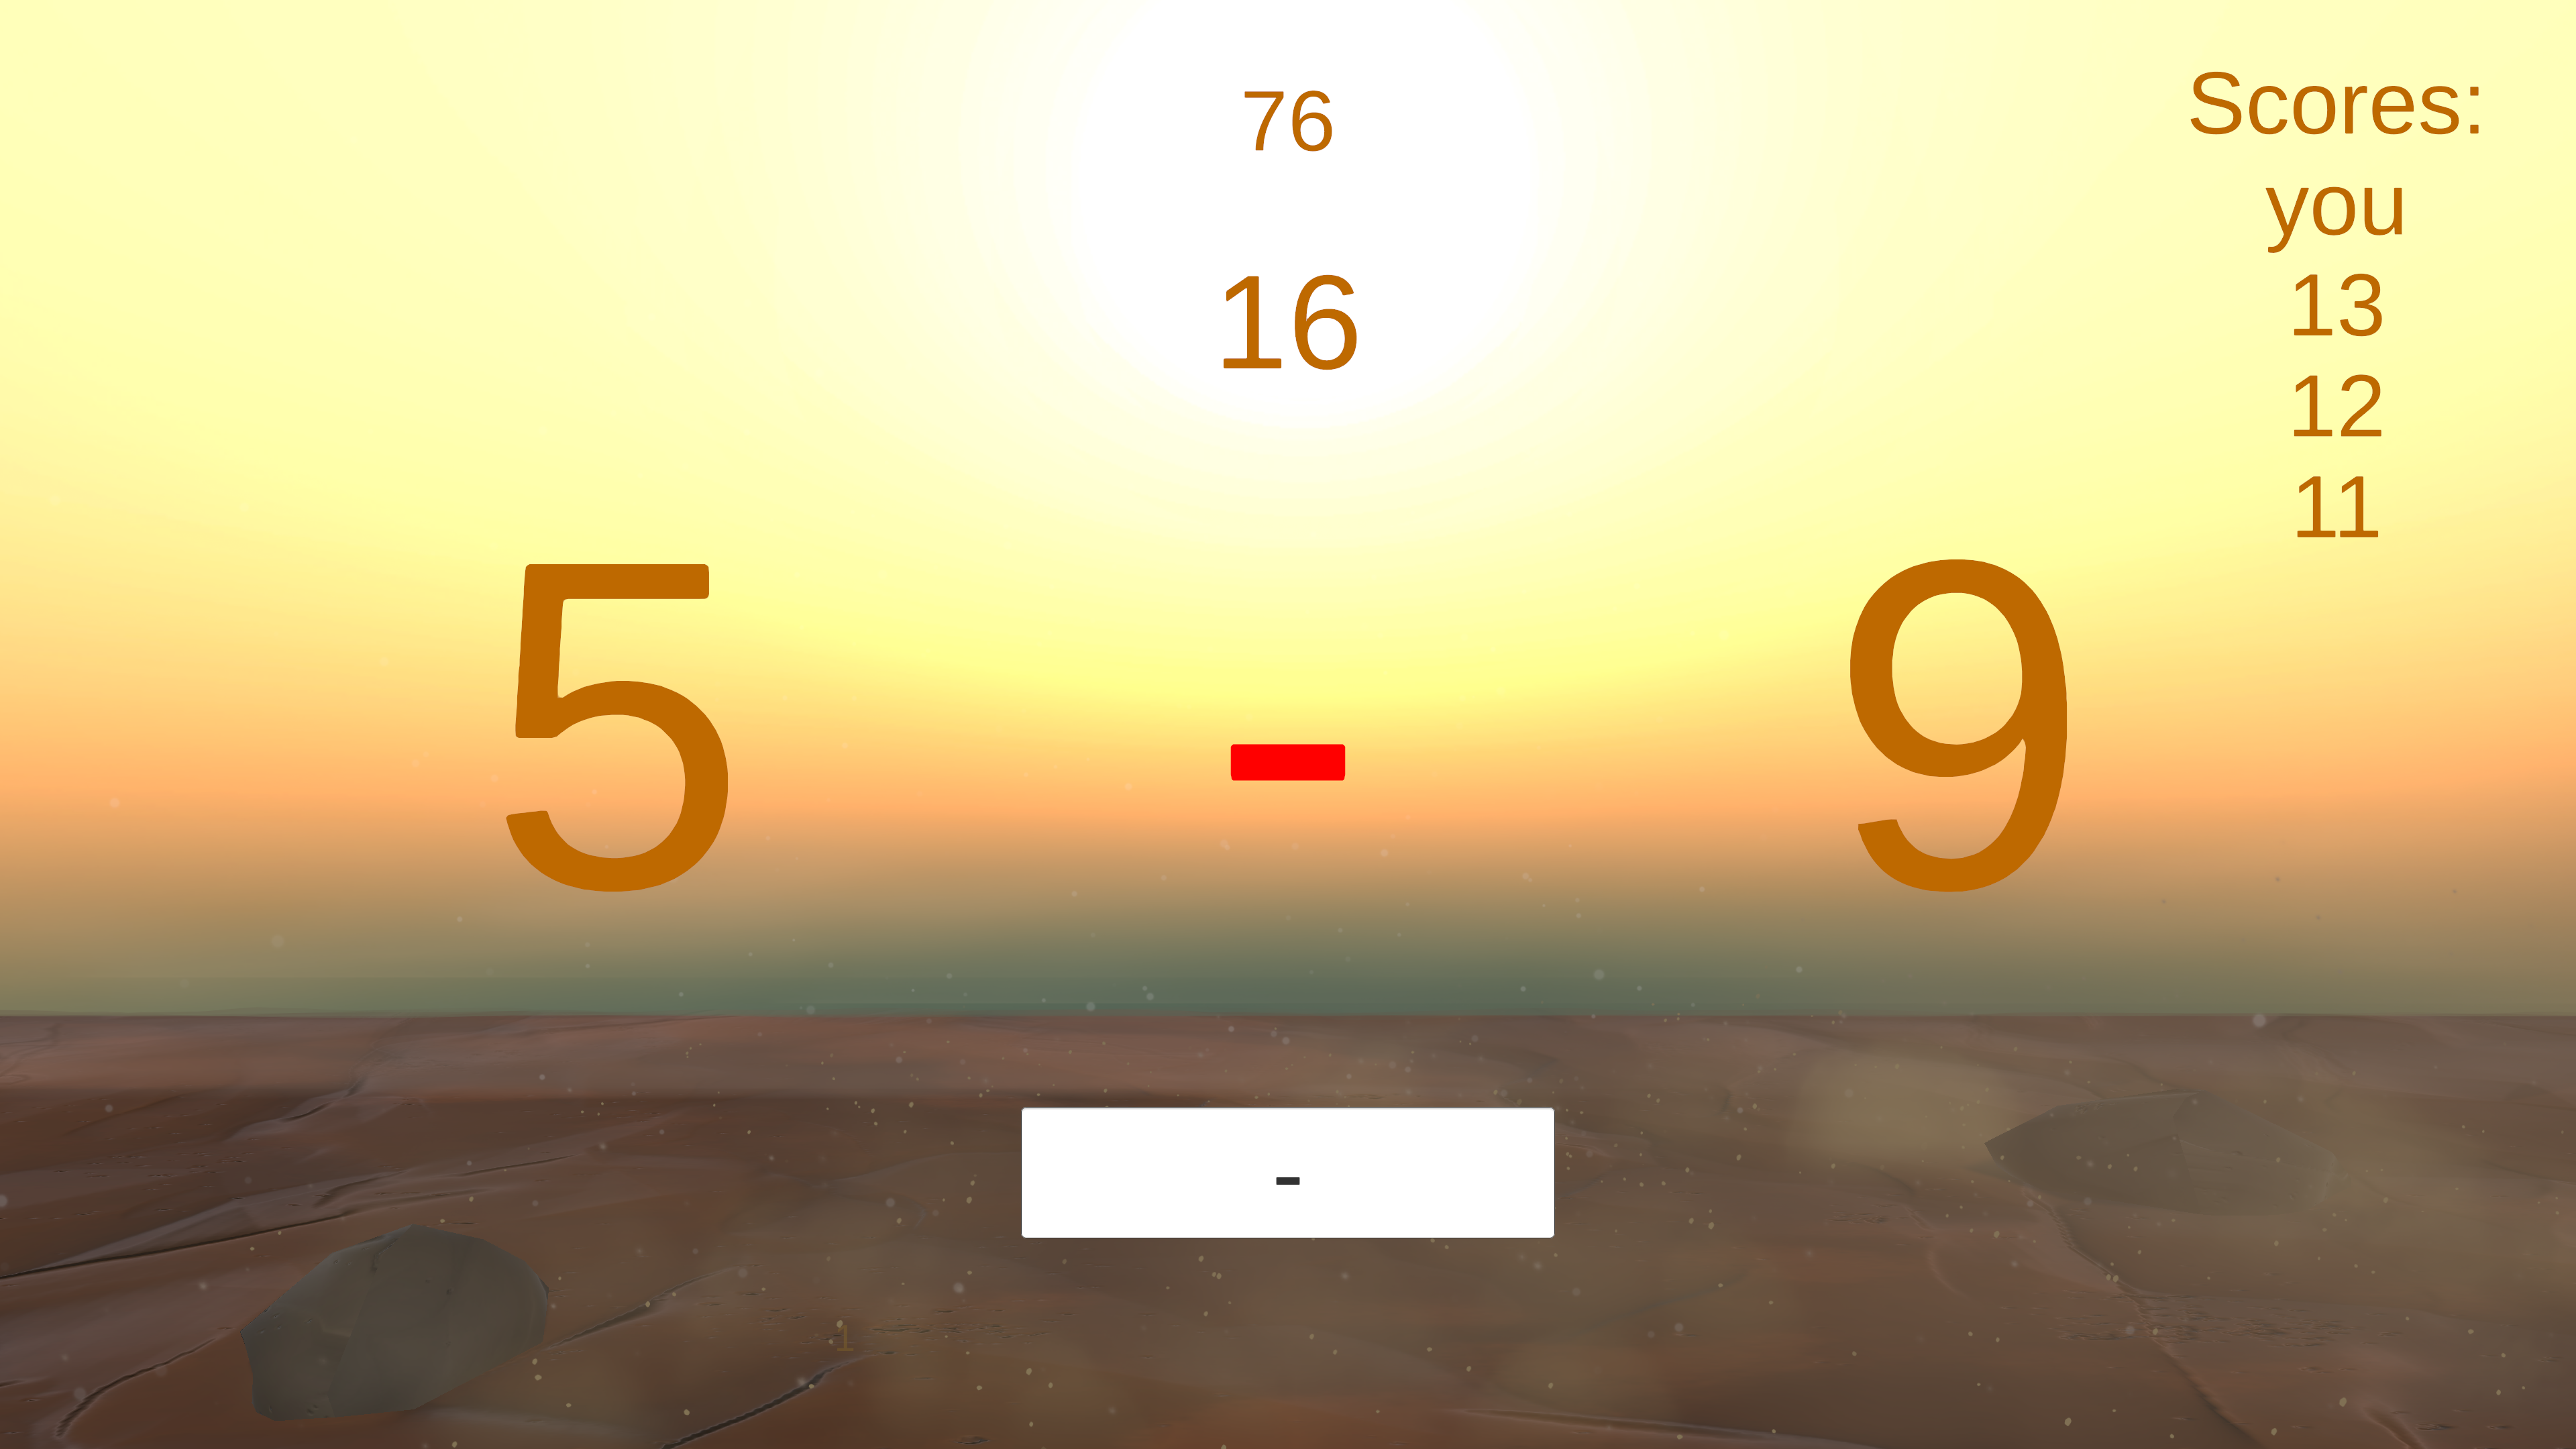
\includegraphics[width=(\linewidth)]{party}
		\caption{Party}
		\label{fig:party}
	\end{subfigure}	
	\caption{Bildschrimaufnahme der Modi}
    \label{fig:modi}
\end{figure}

\begin{figure}[b]
	\centering
    \begin{subfigure}[a]{0.3\linewidth}
    	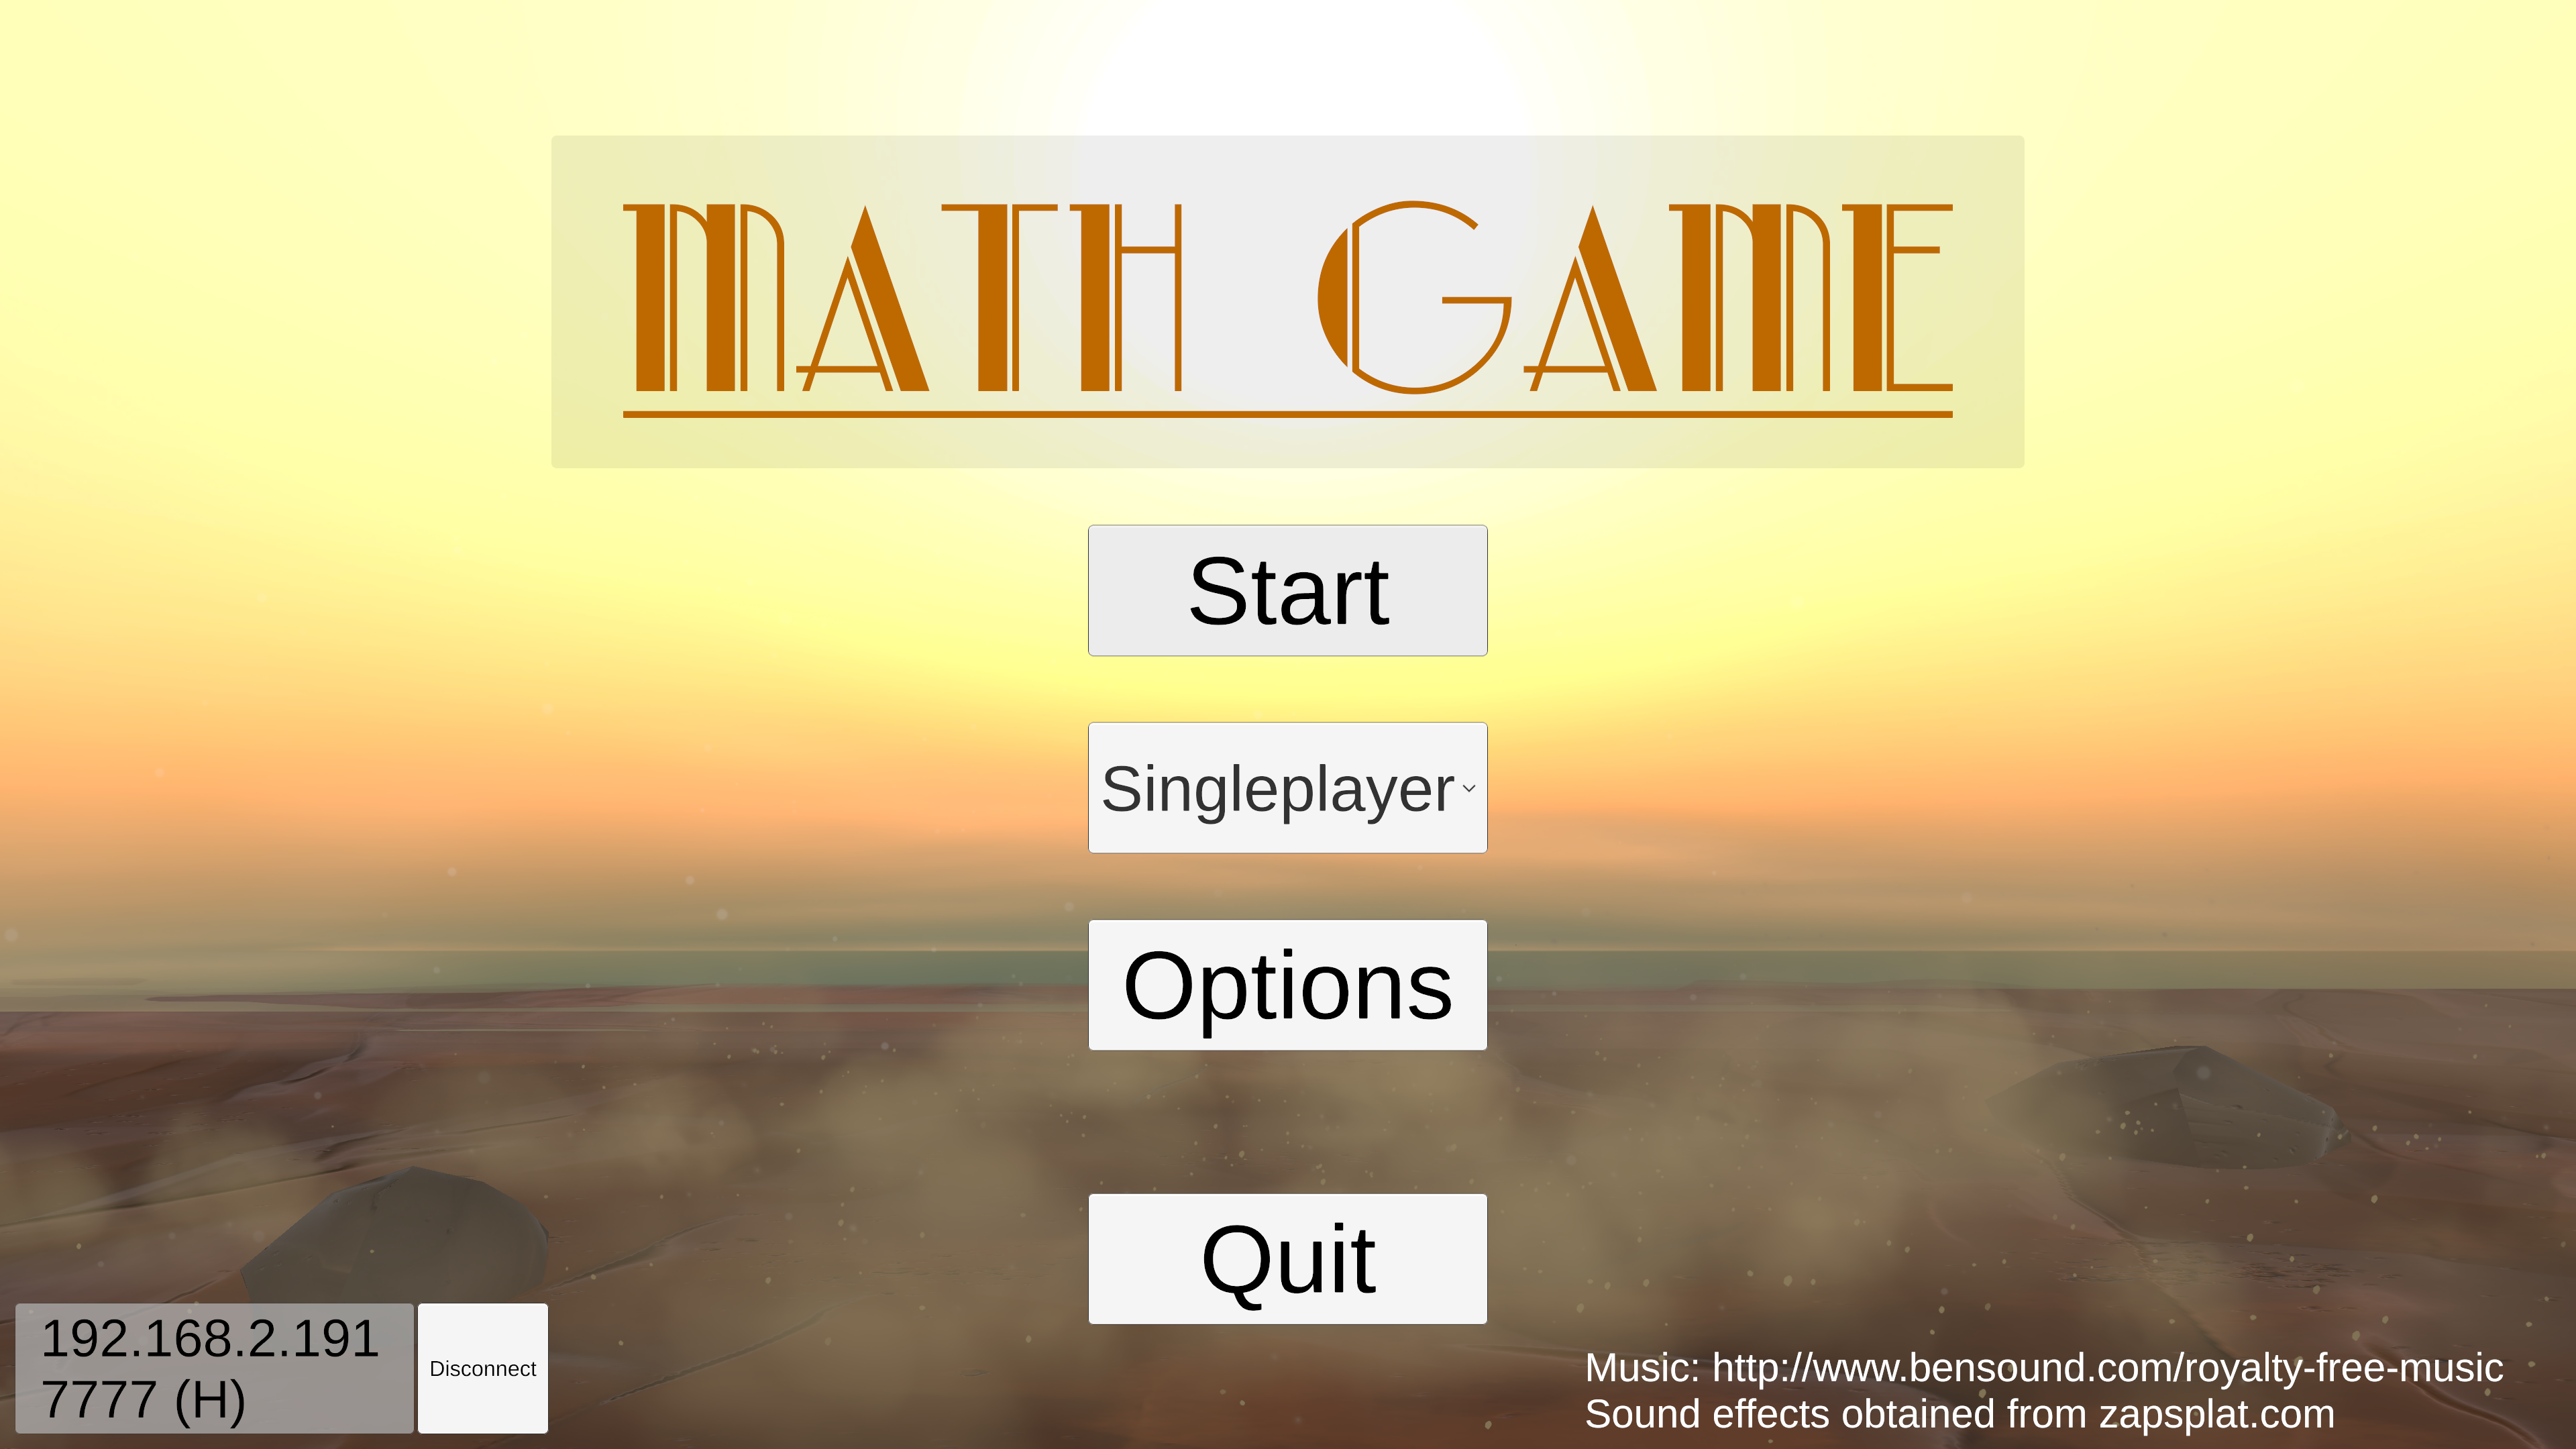
\includegraphics[width=\linewidth]{mainmenuhost}
    	\caption{Ansicht als Host}
        \label{fig:menuhost}
    \end{subfigure}
    \begin{subfigure}[a]{0.3\linewidth}
    	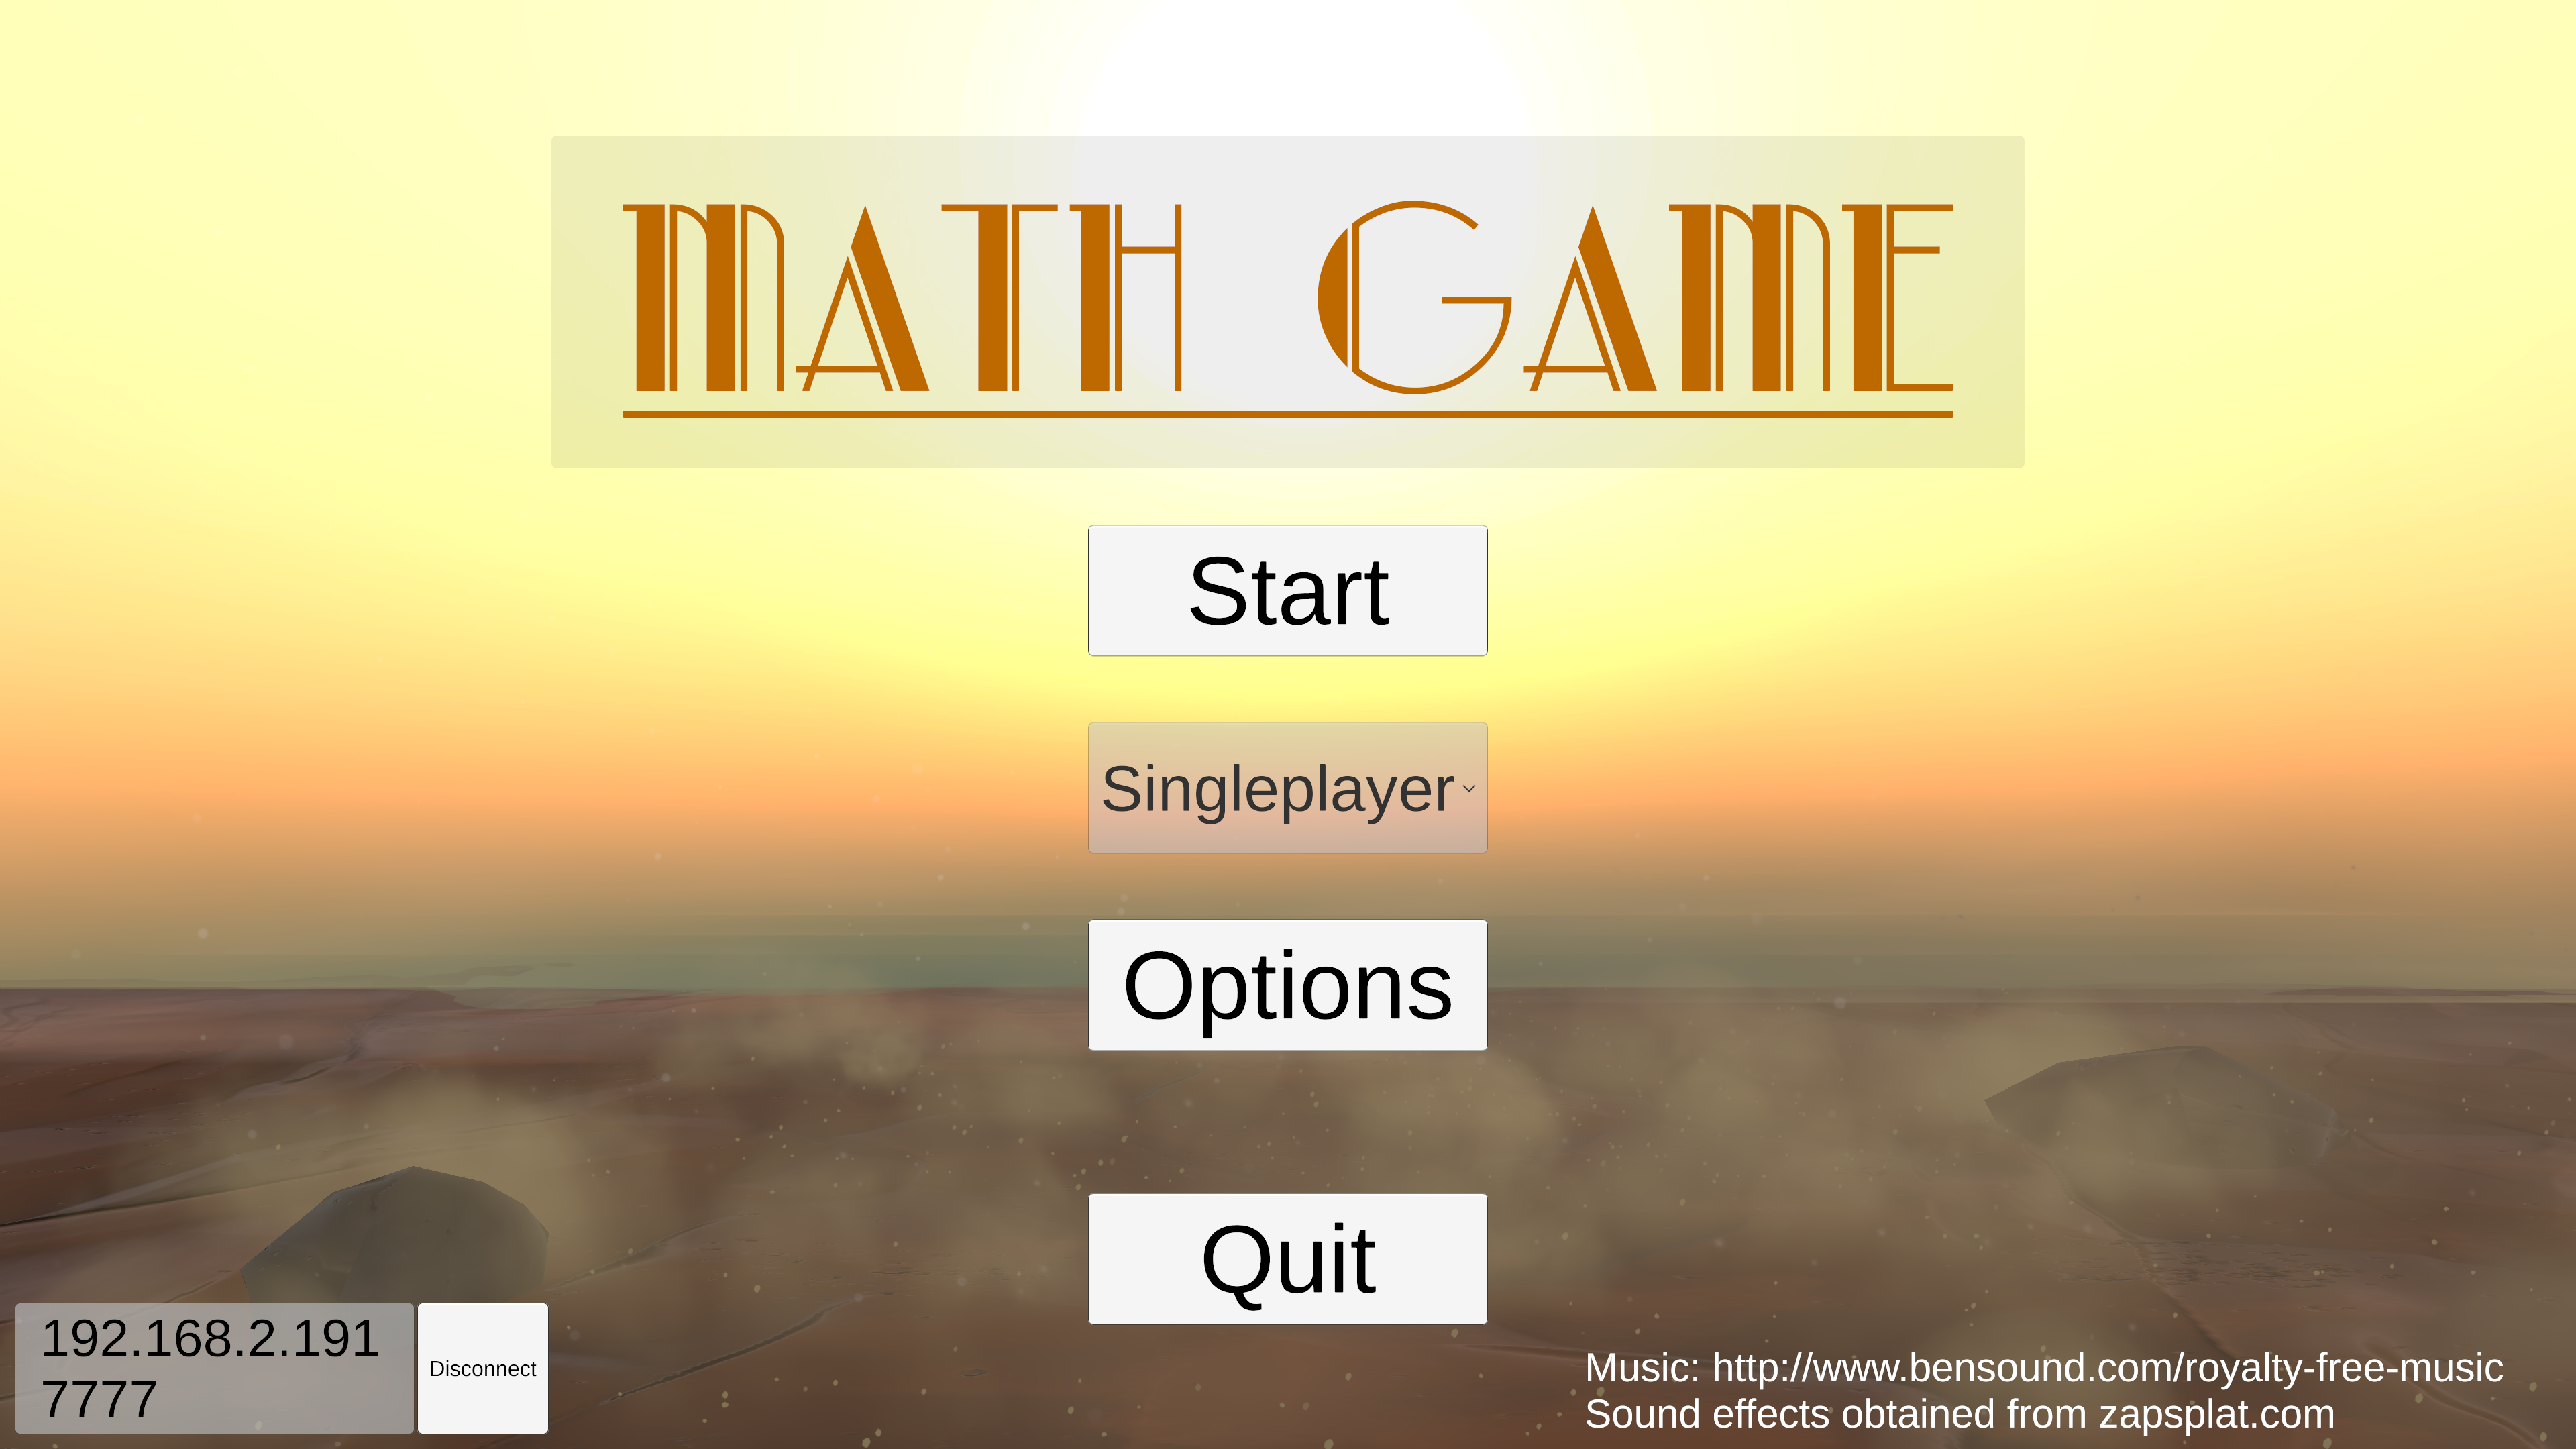
\includegraphics[width=\linewidth]{mainmenuclient}
    	\caption{Ansicht als Client}
        \label{fig:menuclient}
    \end{subfigure}
    \begin{subfigure}[a]{0.3\linewidth}
    	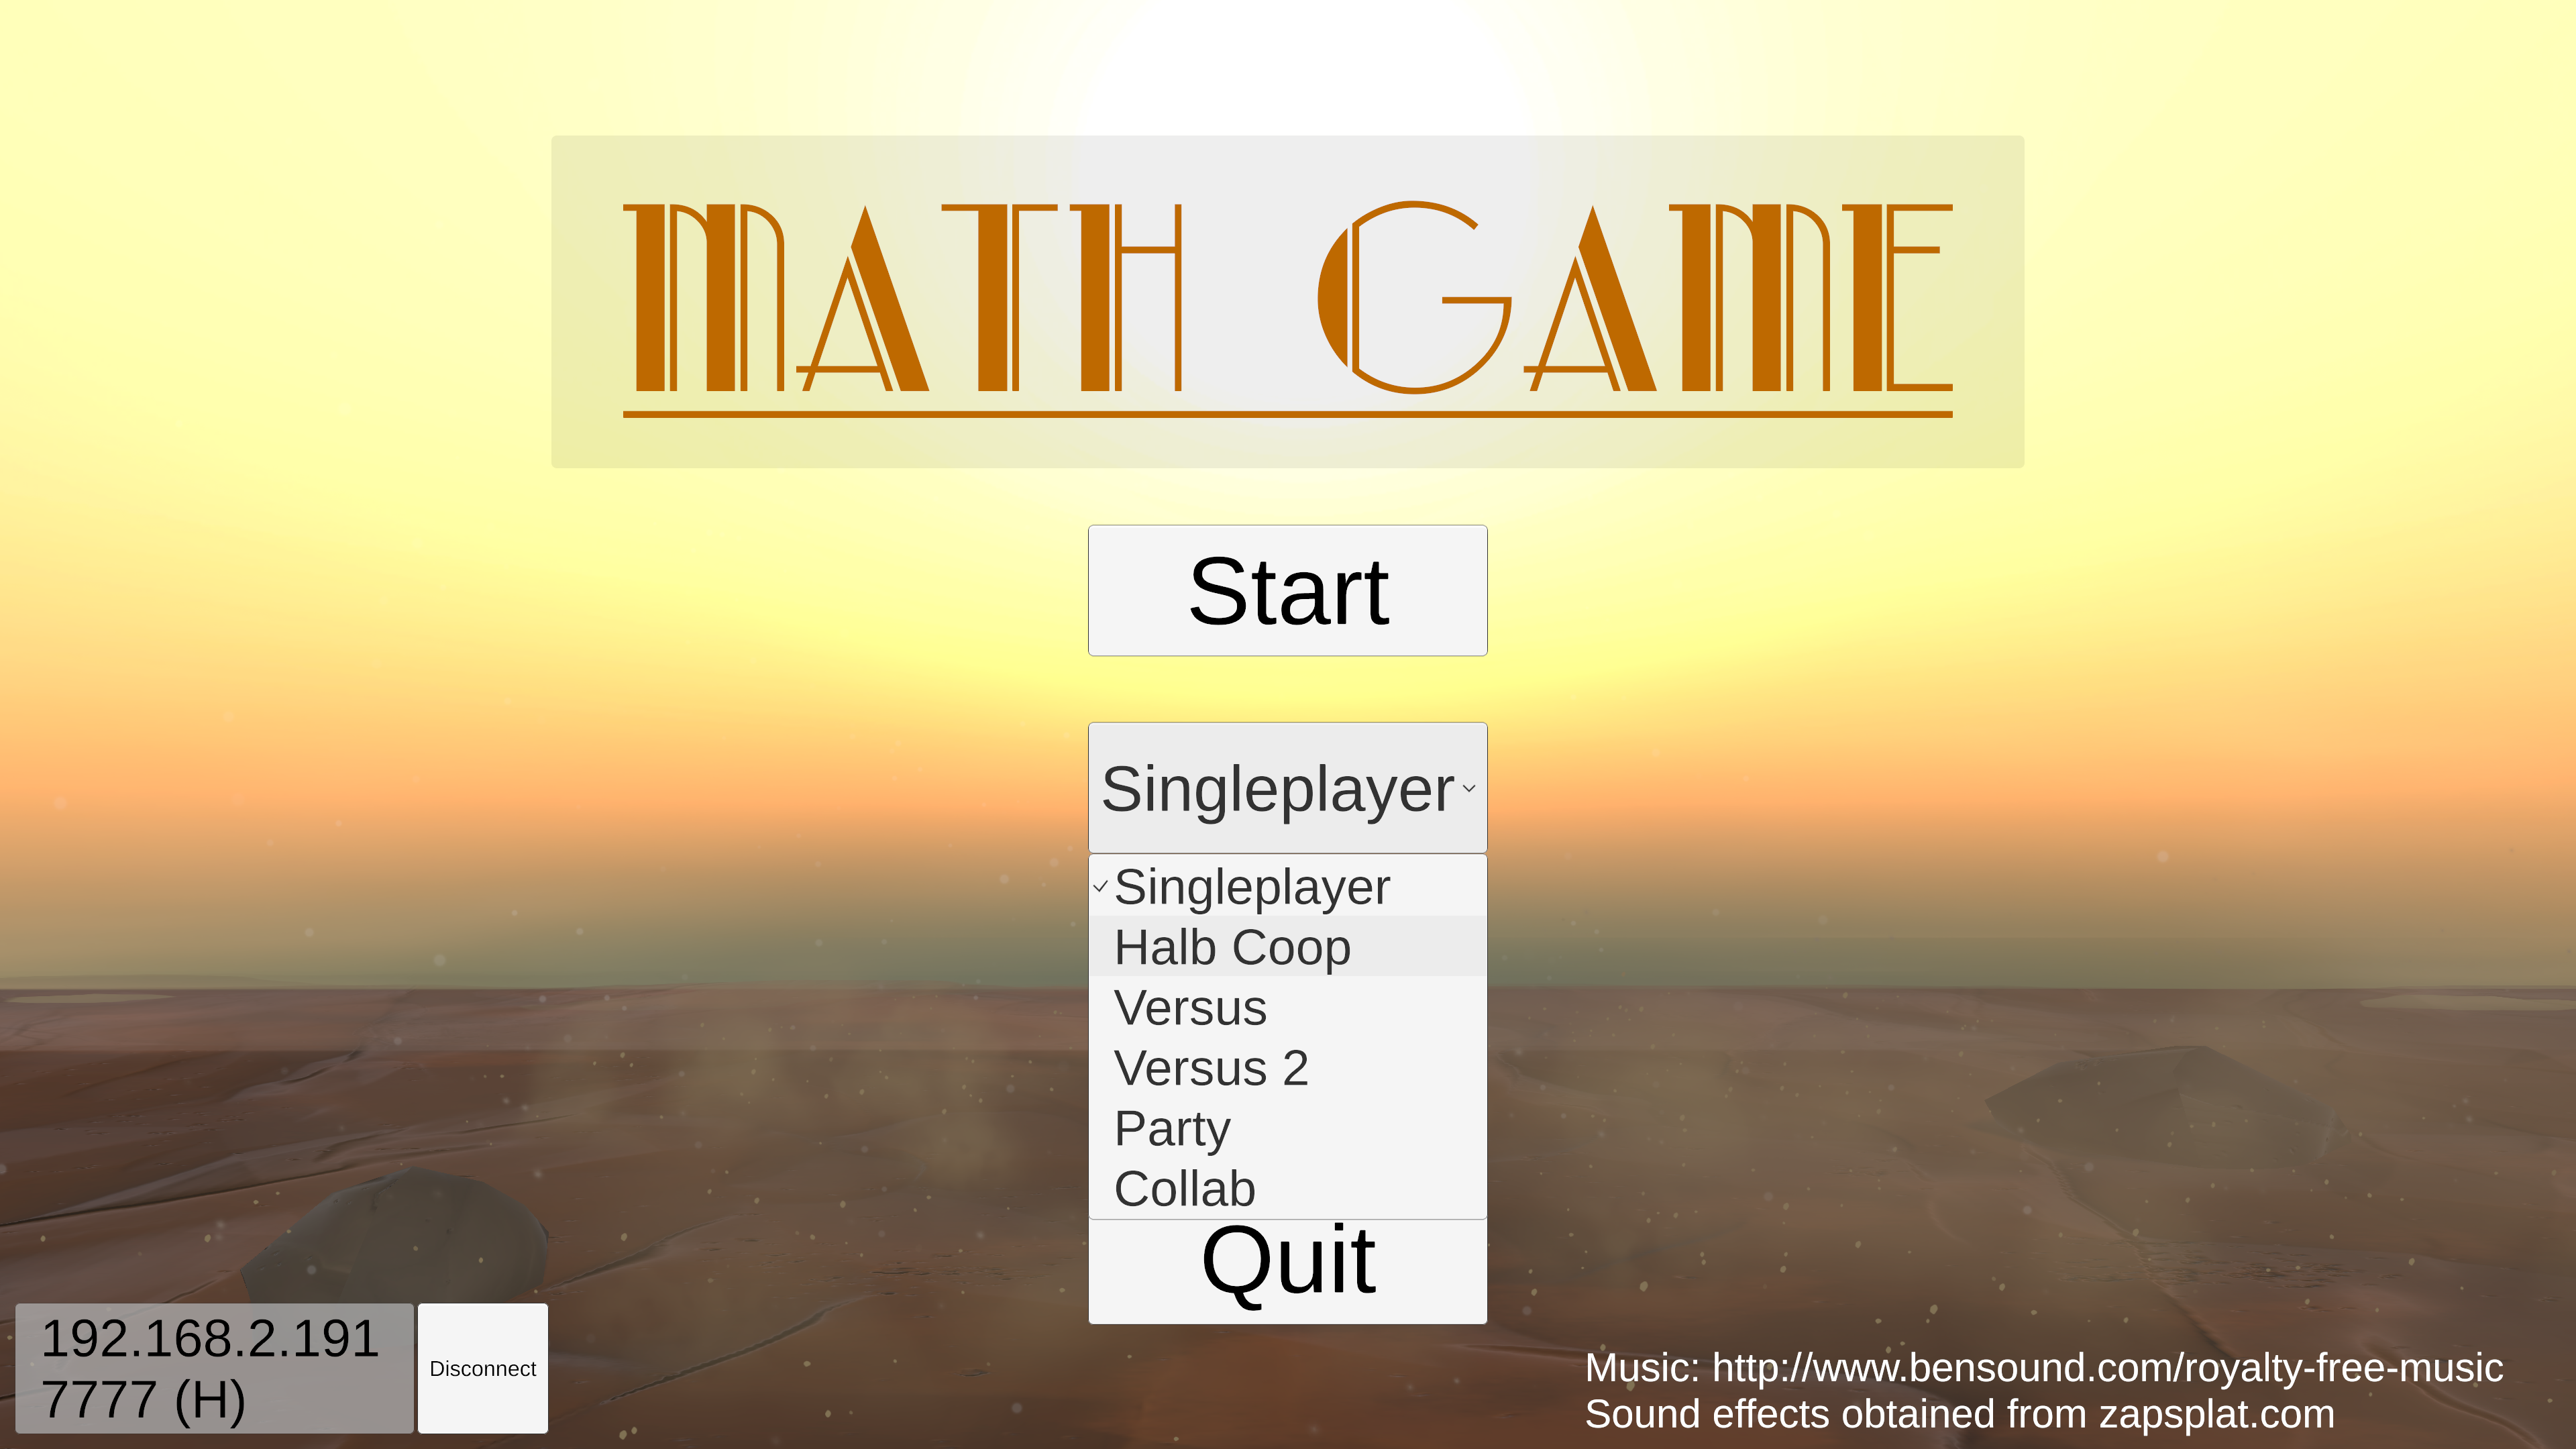
\includegraphics[width=\linewidth]{dropdownmenumodi}
    	\caption{Ansicht bei Wahl des Modus}
        \label{fig:menumodi}
    \end{subfigure}
    \caption{Ansichten des Hauptmenüs}
    \label{menu}
\end{figure}

\begin{wrapfigure}{r}{0.3\textwidth}
	\centering
	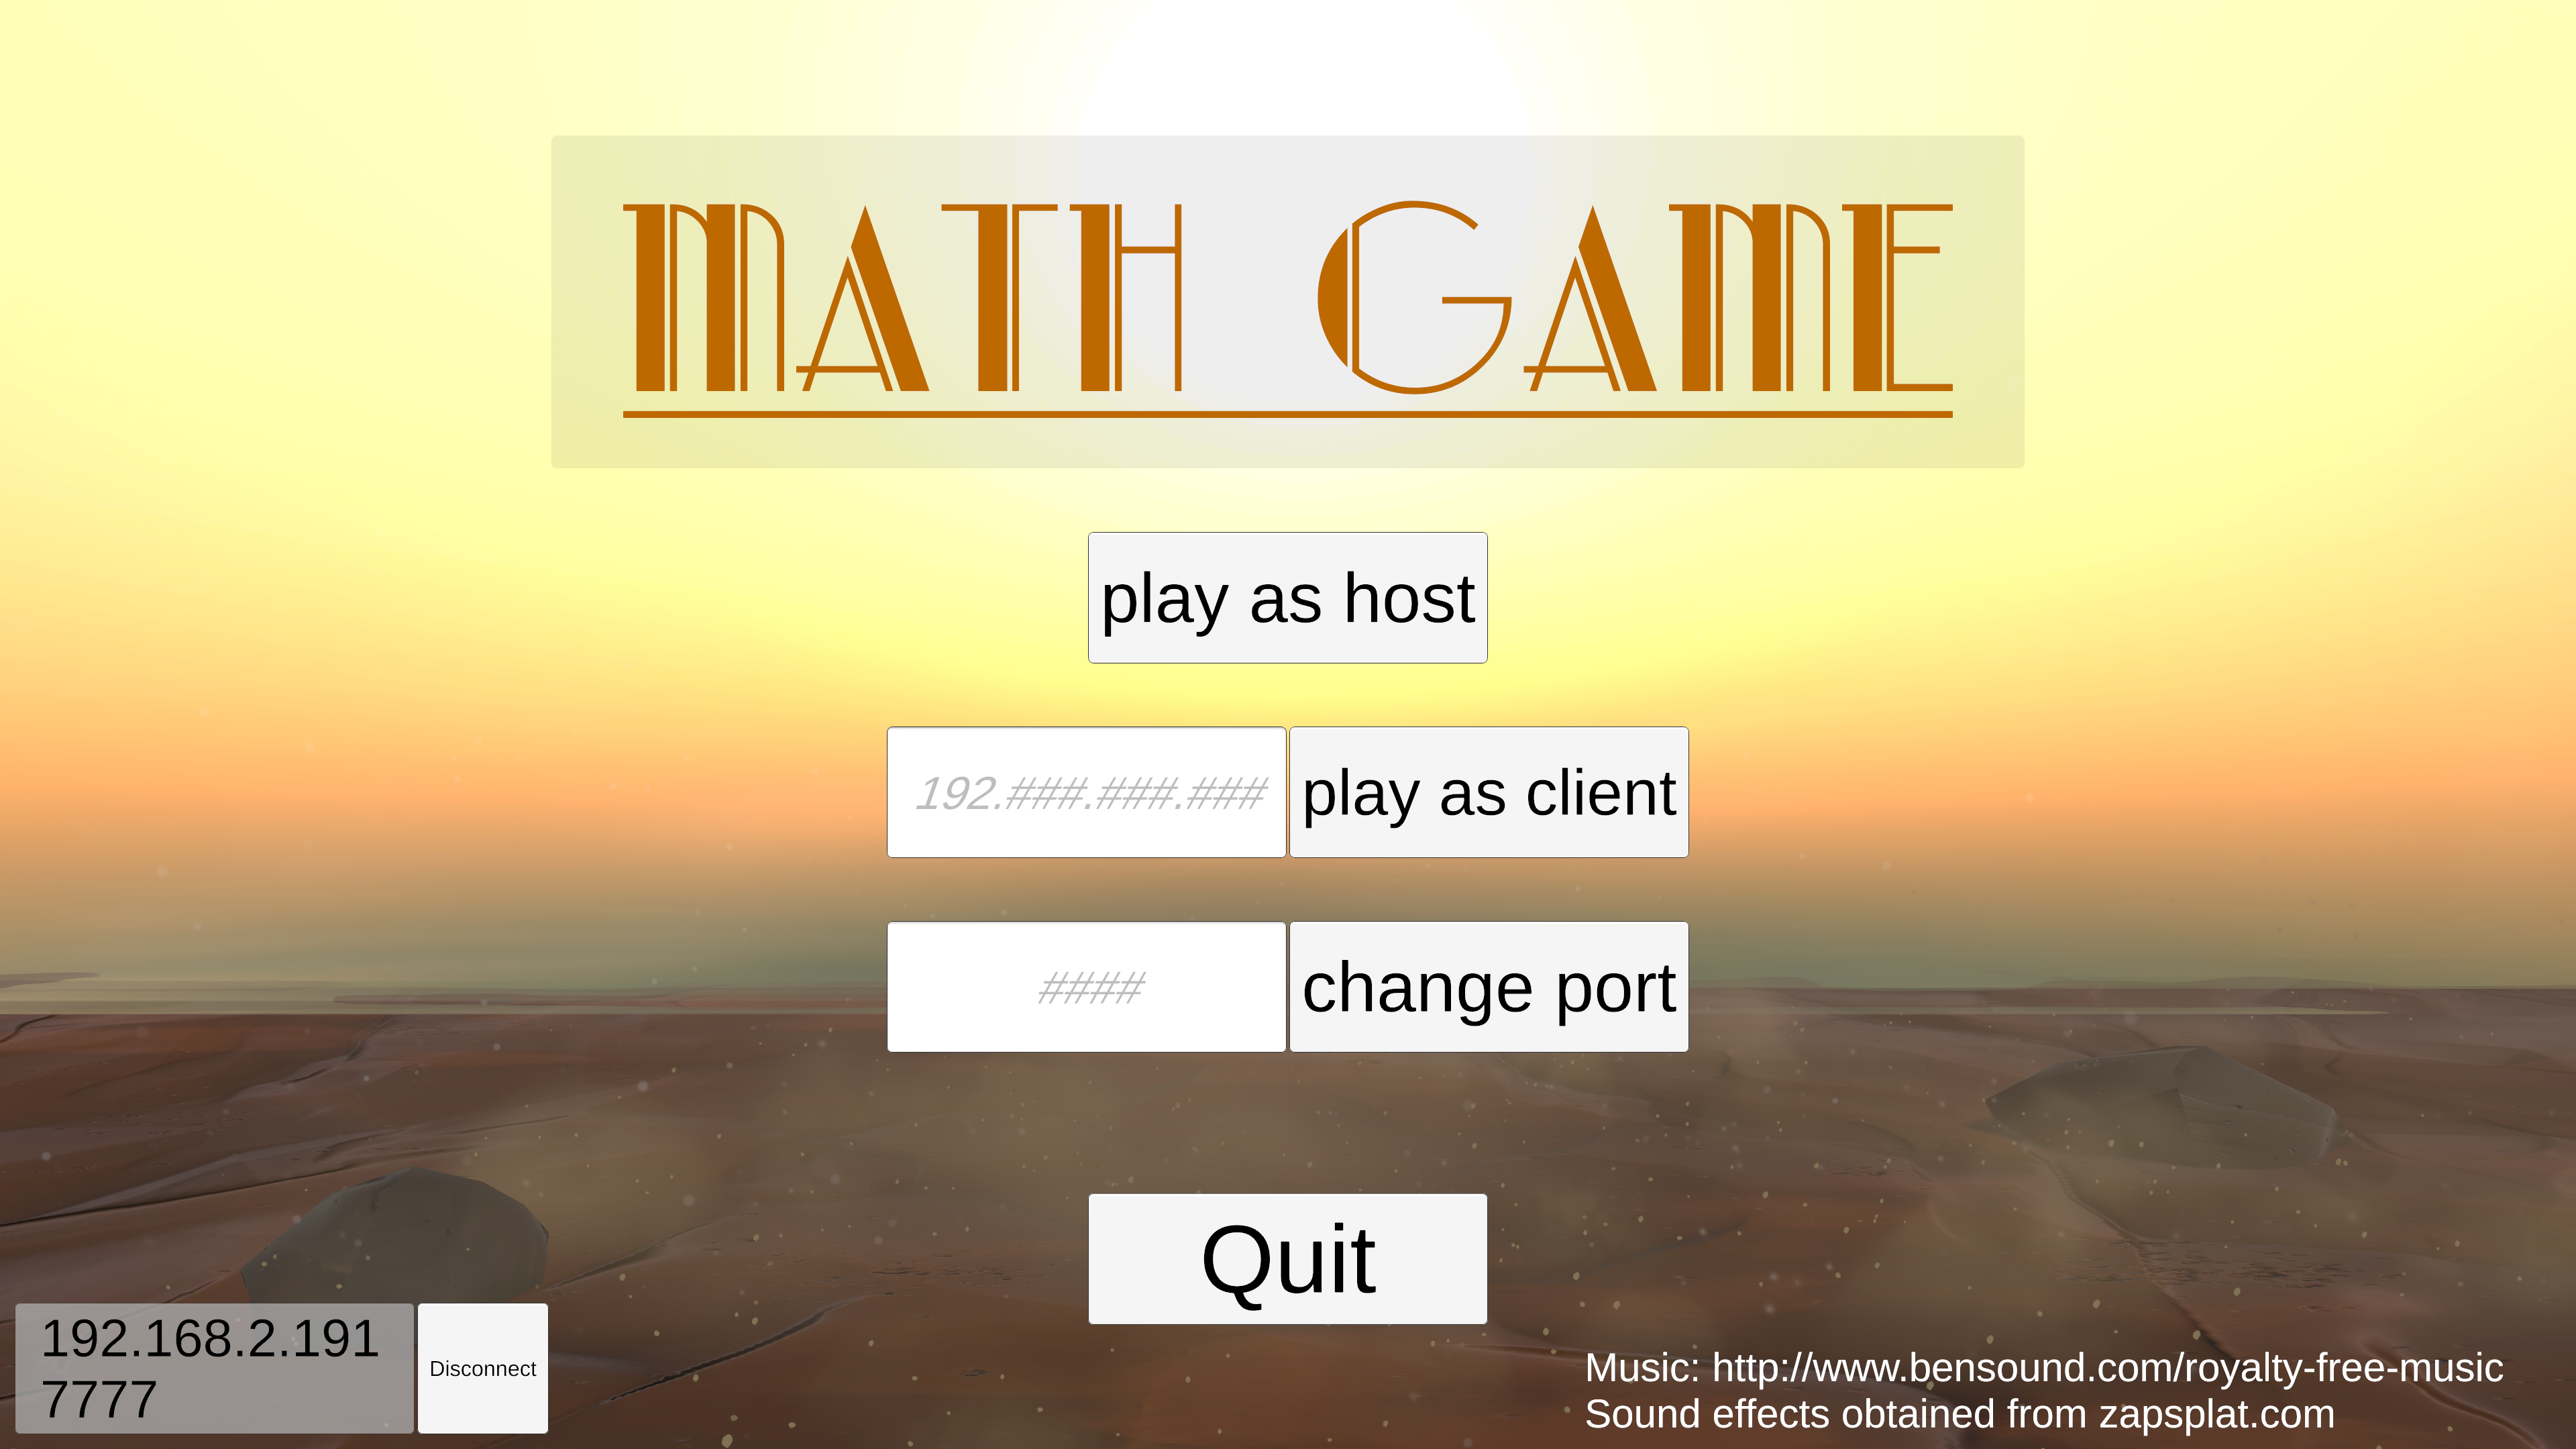
\includegraphics[width=0.3\textwidth]{networkmenu}
    \caption{Netwerkmenü}
   \label{network}
\end{wrapfigure}

\begin{wrapfigure}{r}{0.3\textwidth}
	\centering
    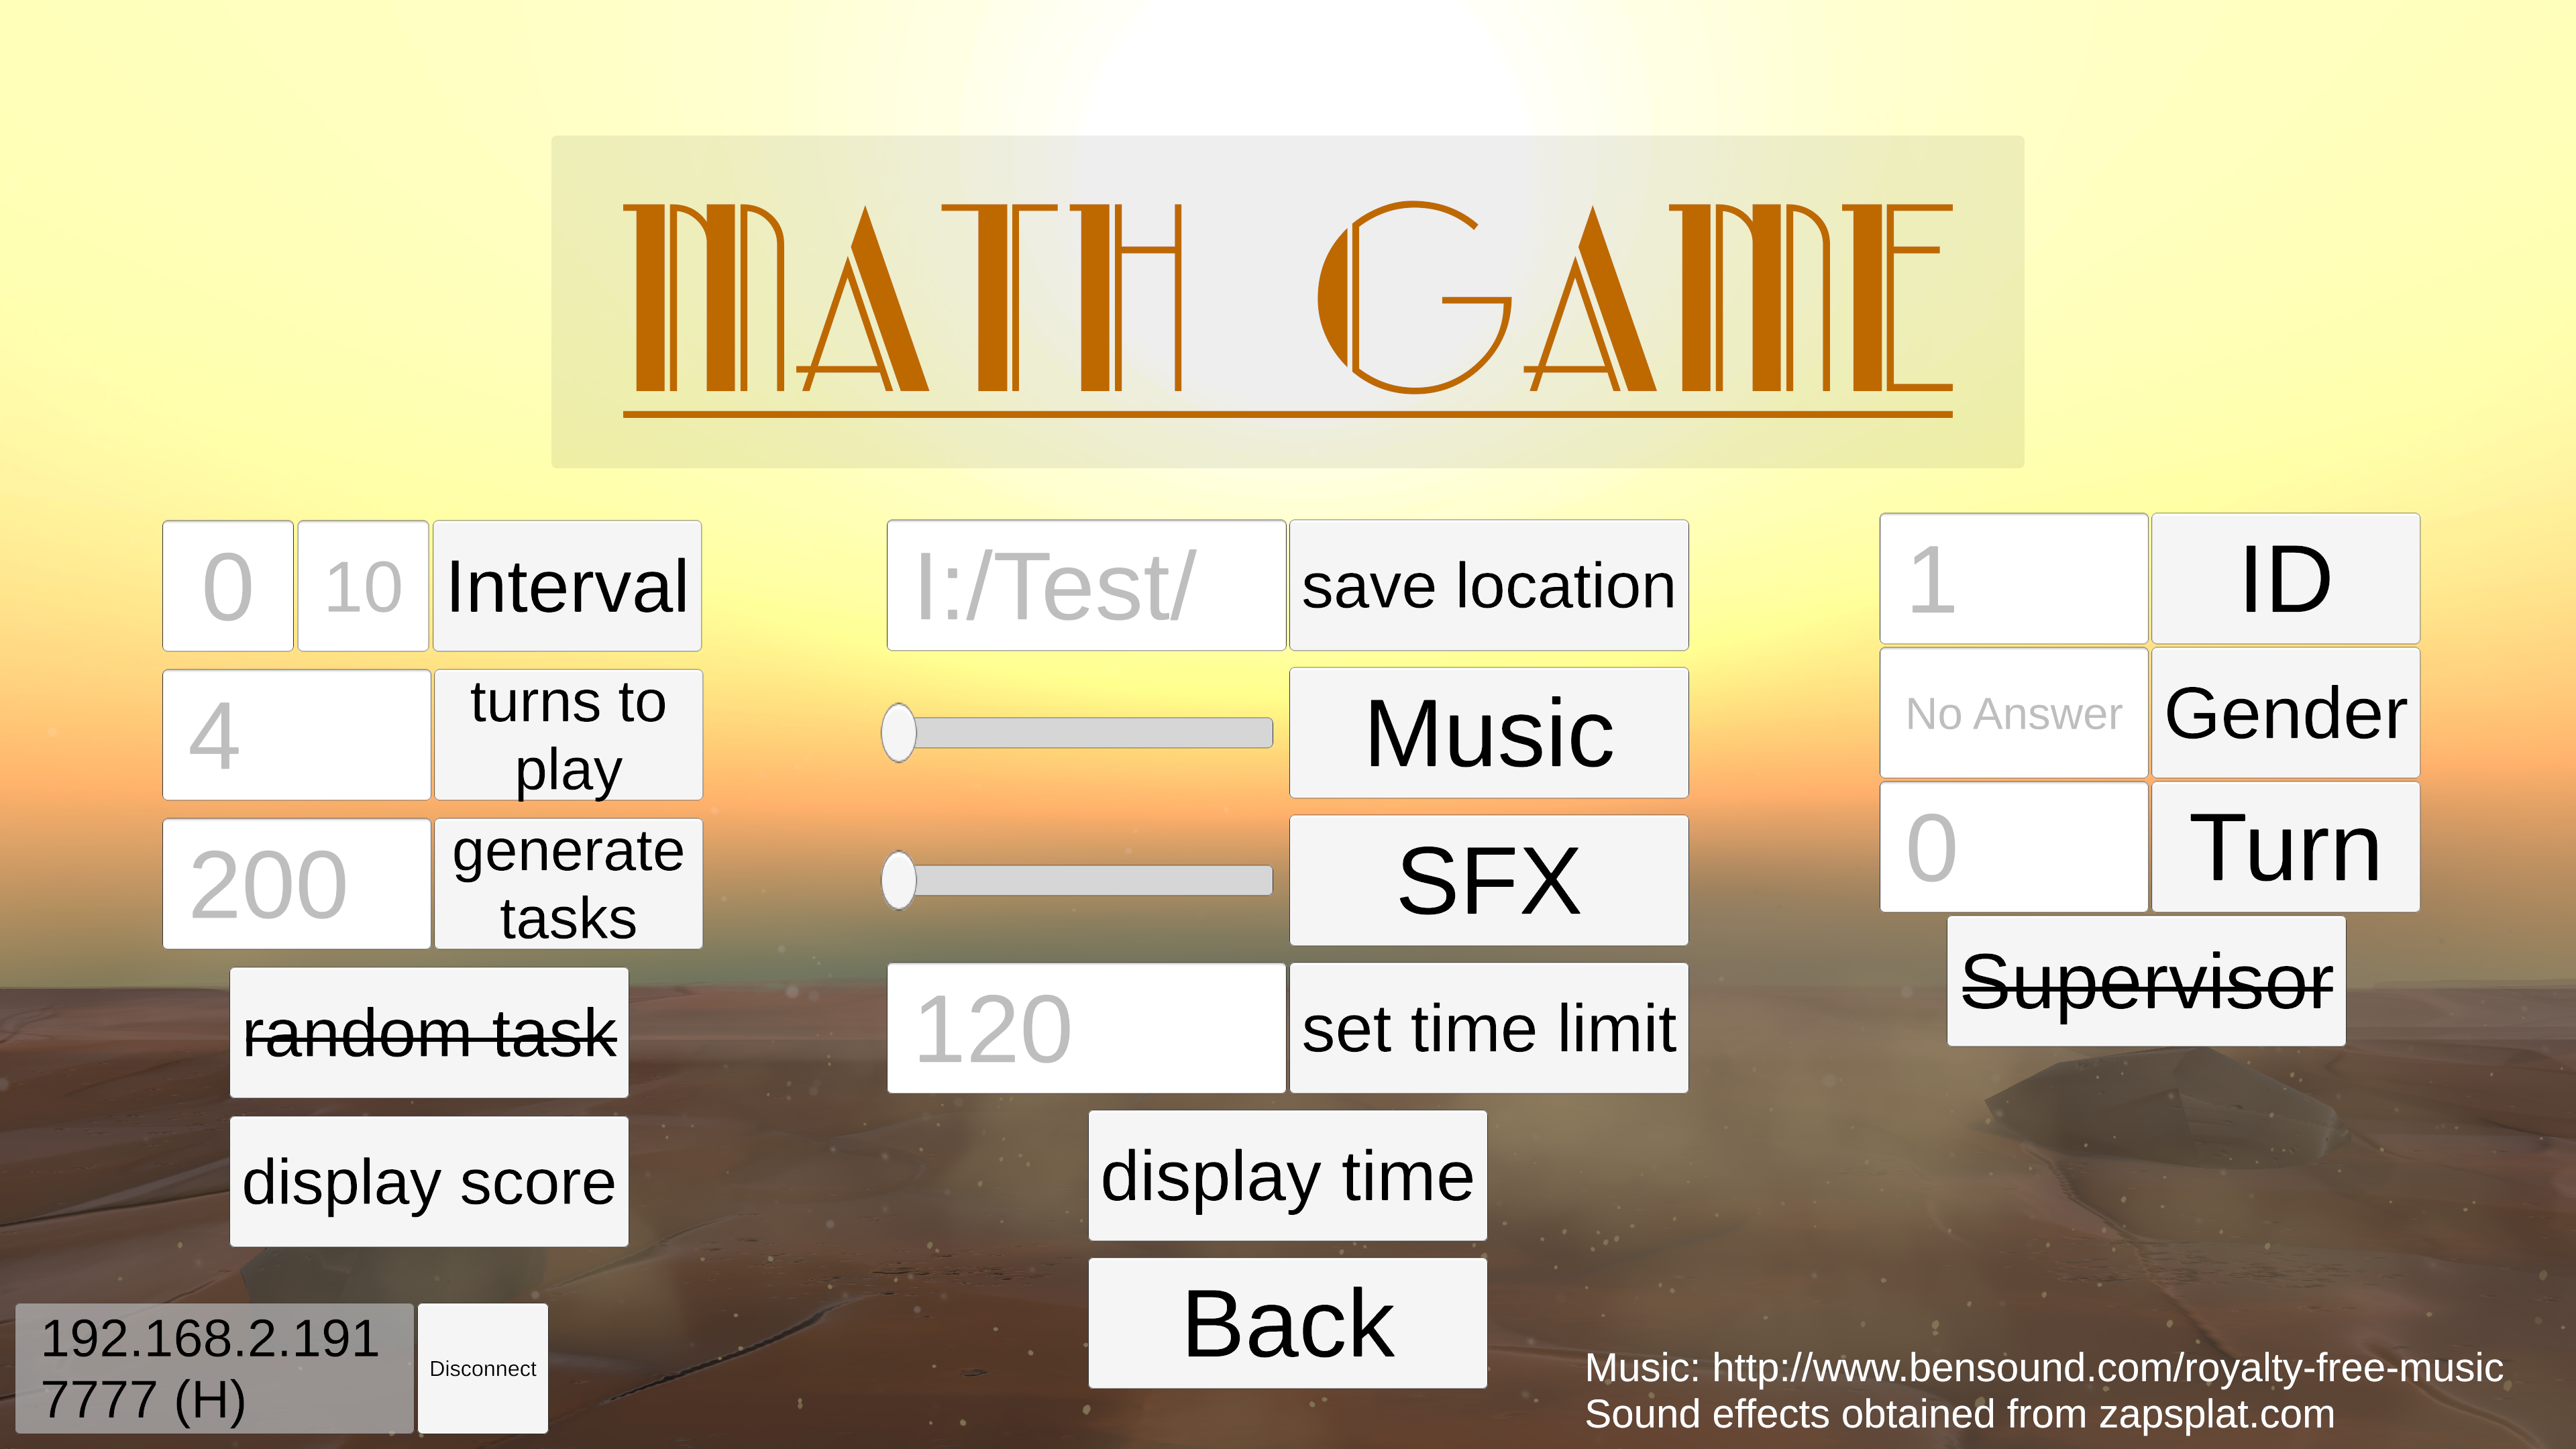
\includegraphics[width=0.3\textwidth]{optionsmenu}
    \caption{Optionen}
    \label{option}
\end{wrapfigure}
%

\bibliography{Bibliographie}
\listoffigures
%\appendix{}
%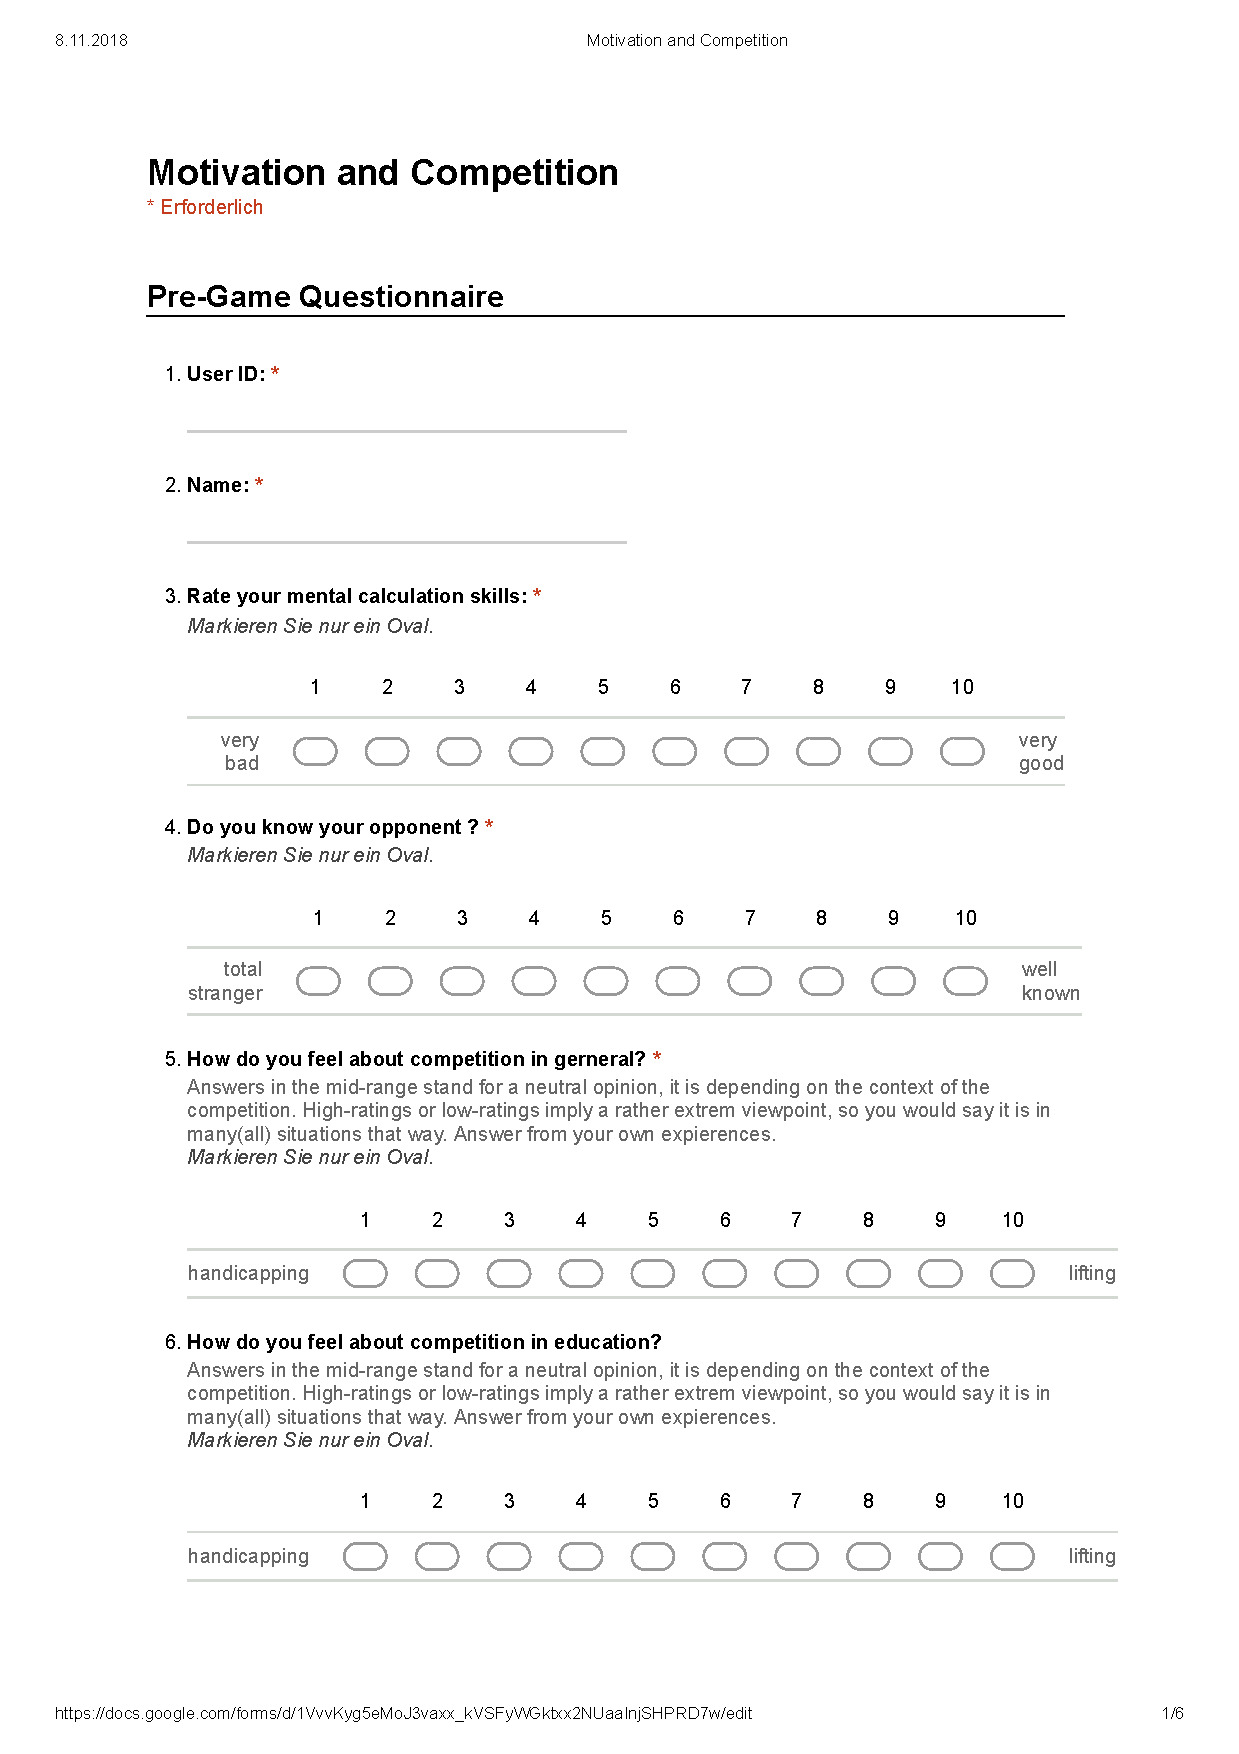
\includepdf[pages=-]{./Ressourcen/questionnaire.pdf}

\end{document}
